\documentclass[output=paper]{langsci/langscibook} 
\title{Maltese}  

\author{Christopher Lucas\affiliation{SOAS University of London}\lastand 
 Slavomír Čéplö\affiliation{Institute of Oriental Studies, Slovak Academy of Sciences / IMAFO Abteilung Byzanzforschung, Österreichische Akademie der Wissenschaften}
}

\abstract{
This chapter presents an overview of the most prominent contact-induced developments in the history of Maltese, a language which is genetically a variety of Arabic, but which has undergone significant changes, largely as a result of lengthy contact with Sicilian, Italian, and English. We first address the precise affiliation of Maltese and the nature of the historical and ongoing contact situations, before detailing relevant developments in the realms of phonology, inflectional and derivational morphology, syntax and lexicon.
}

% \IfFileExists{../localcommands.tex}{
%   % add all extra packages you need to load to this file 
\usepackage{graphicx}
\usepackage{tabularx}
\usepackage{amsmath} 
\usepackage{multicol}
\usepackage{lipsum}
\usepackage[stable]{footmisc}
\usepackage{adforn}
%%%%%%%%%%%%%%%%%%%%%%%%%%%%%%%%%%%%%%%%%%%%%%%%%%%%
%%%                                              %%%
%%%           Examples                           %%%
%%%                                              %%%
%%%%%%%%%%%%%%%%%%%%%%%%%%%%%%%%%%%%%%%%%%%%%%%%%%%%
% remove the percentage signs in the following lines
% if your book makes use of linguistic examples
\usepackage{./langsci/styles/langsci-optional} 
\usepackage{./langsci/styles/langsci-lgr}
\usepackage{morewrites} 
%% if you want the source line of examples to be in italics, uncomment the following line
% \def\exfont{\it}

\usepackage{enumitem}
\newlist{furtherreading}{description}{1}
\setlist[furtherreading]{font=\normalfont,labelsep=\widthof{~},noitemsep,align=left,leftmargin=\parindent,labelindent=0pt,labelwidth=-\parindent}
\usepackage{phonetic}
\usepackage{chronosys,tabularx}
\usepackage{csquotes}
\usepackage[stable]{footmisc} 

\usepackage{langsci-bidi}
\usepackage{./langsci/styles/langsci-gb4e} 

%   \makeatletter
\let\thetitle\@title
\let\theauthor\@author 
\makeatother

\newcommand{\togglepaper}[1][0]{ 
  \bibliography{../localbibliography}
  \papernote{\scriptsize\normalfont
    \theauthor.
    \thetitle. 
    To appear in: 
    Christopher Lucas and Stefano Manfredi (eds.),  
    Arabic and contact-induced language change
    Berlin: Language Science Press. [preliminary page numbering]
  }
  \pagenumbering{roman}
  \setcounter{chapter}{#1}
  \addtocounter{chapter}{-1}
}

\newfontfamily\Parsifont[Script=Arabic]{ScheherazadeRegOT_Jazm.ttf} 
\newcommand{\arabscript}[1]{\RL{\Parsifont #1}}
\newcommand{\textarabic}[1]{{\arabicfont #1}}

\newcommand{\textstylest}[1]{{\color{red}#1}}

\patchcmd{\mkbibindexname}{\ifdefvoid{#3}{}{\MakeCapital{#3}
}}{\ifdefvoid{#3}{}{#3 }}{}{\AtEndDocument{\typeout{mkbibindexname could
not be patched.}}}

%command for italic r with dot below with horizontal correction to put the dot in the prolongation of the vertical stroke
%for some reason, the dot is larger than expected, so we explicitly reduce the font size (to \small)
%for the time being, the font is set to an absolute value. To be more robust, a relative reduction would be better, but this might not be required right now
\newcommand{\R}{r\kern-.05ex{\small{̣}}\kern.05ex}


\DeclareLabeldate{%
    \field{date}
    \field{year}
    \field{eventdate}
    \field{origdate}
    \field{urldate}
    \field{pubstate}
    \literal{nodate}
}

\renewbibmacro*{addendum+pubstate}{% Thanks to https://tex.stackexchange.com/a/154367 for the idea
  \printfield{addendum}%
  \iffieldequalstr{labeldatesource}{pubstate}{}
  {\newunit\newblock\printfield{pubstate}}
}
 
%   %% hyphenation points for line breaks
%% Normally, automatic hyphenation in LaTeX is very good
%% If a word is mis-hyphenated, add it to this file
%%
%% add information to TeX file before \begin{document} with:
%% %% hyphenation points for line breaks
%% Normally, automatic hyphenation in LaTeX is very good
%% If a word is mis-hyphenated, add it to this file
%%
%% add information to TeX file before \begin{document} with:
%% %% hyphenation points for line breaks
%% Normally, automatic hyphenation in LaTeX is very good
%% If a word is mis-hyphenated, add it to this file
%%
%% add information to TeX file before \begin{document} with:
%% \include{localhyphenation}
\hyphenation{
affri-ca-te
affri-ca-tes
com-ple-ments
homo-phon-ous
start-ed
Meso-potam-ian
morpho-phono-logic-al-ly
morpho-phon-em-ic-s
Palestin-ian
re-present-ed
Ki-nubi
ḥawār-iyy-ūn
archa-ic-ity
fuel-ed
de-velop-ment
pros-od-ic
Arab-ic
in-duced
phono-logy
possess-um
possess-ive-s
templ-ate
spec-ial
espec-ial-ly
nat-ive
pass-ive
clause-s
potent-ial-ly
Lusignan
commun-ity
tobacco
posi-tion
Cushit-ic
Middle
with-in
re-finit-iz-ation
langu-age-s
langu-age
diction-ary
glossary
govern-ment
eight
counter-part
nomin-al
equi-valent
deont-ic
ana-ly-sis
Malt-ese
un-fortun-ate-ly
scient-if-ic
Catalan
Occitan
ḥammāl
cross-linguist-ic-al-ly
predic-ate
major-ity
ignor-ance
chrono-logy
south-western
mention-ed
borrow-ed
neg-ative
de-termin-er
European
under-mine
detail
Oxford
Socotra
numer-ous
spoken
villages
nomad-ic
Khuze-stan
Arama-ic
Persian
Ottoman
Ottomans
Azeri
rur-al
bi-lingual-ism
borrow-ing
prestig-ious
dia-lects
dia-lect
allo-phone
allo-phones
poss-ible
parallel
parallels
pattern
article
common-ly
respect-ive-ly
sem-antic
Moroccan
Martine
Harrassowitz
Grammatic-al-ization
grammatic-al-ization
Afro-asiatica
Afro-asiatic
continu-ation
Semit-istik
varieties
mono-phthong
mono-phthong-ized
col-loquial
pro-duct
document-ary
ex-ample-s
ex-ample
termin-ate
element-s
Aramaeo-grams
Centr-al
idioms
Arab-ic
Dadan-it-ic
sub-ordin-ator
Thamud-ic
difficult
common-ly
Revue
Bovingdon
under
century
attach
attached
bundle
graph-em-ic
graph-emes
cicada
contrast-ive
Corriente
Andalusi
Kossmann
morpho-logic-al
inter-action
dia-chroniques
islámica
occid-ent-al-ismo
dialecto-logie
Reichert
coloni-al
Milton
diphthong-al
linguist-ic
linguist-ics
affairs
differ-ent
phonetic-ally
kilo-metres
stabil-ization
develop-ments
in-vestig-ation
Jordan-ian
notice-able
level-ed
migrants
con-dition-al
certain-ly
general-ly
especial-ly
af-fric-ation
Jordan
counter-parts
com-plication
consider-ably
inter-dent-al
com-mun-ity
inter-locutors
com-pon-ent
region-al
socio-historical
society
simul-taneous
phon-em-ic
roman-ization
Classic-al
funeral
Kurmanji
pharyn-geal-ization
vocab-ulary
phon-et-ic
con-sonant
con-sonants
special-ized
latter
latters
in-itial
ident-ic-al
cor-relate
geo-graphic-al-ly
Öpengin
Kurd-ish
in-digen-ous
sunbul
Christ-ian
Christ-ians
sekin-în
fatala
in-tegration
dia-lect-al
Matras
morpho-logy
in-tens-ive
con-figur-ation
im-port-ant
com-plement
ḥaddād
e-merg-ence
Benjmamins
struct-ure
em-pir-ic-al
Orient-studien
Anatolia
American
vari-ation
Jastrow
Geoffrey
Yarshater
Ashtiany
Edmund
Mahnaz
En-cyclo-pædia
En-cyclo-paedia
En-cyclo-pedia
Leiden
dia-spora
soph-is-ic-ated
Sasan-ian
every-day
domin-ance
Con-stitu-tion-al
religi-ous
sever-al
Manfredi
re-lev-ance
re-cipi-ent
pro-duct-iv-ity
turtle
Morocco
ferman
Maghreb-ian
algérien
stand-ard
systems
Nicolaï
Mouton
mauritani-en
Gotho-burg-ensis
socio-linguist-ique
plur-al
archiv-al
Arab-ian
drop-ped
dihāt
de-velop-ed
ṣuḥbat
kitāba
kitābat
com-mercial
eight-eenth
region
Senegal
mechan-ics
Maur-itan-ia
Ḥassān-iyya
circum-cision
cor-relation
labio-velar-ization
vowel
vowels
cert-ain
īggīw
series
in-tegrates
dur-ative
inter-dent-als
gen-itive
Tuareg
tălămut
talawmāyət
part-icular
part-icular-ly
con-diment
vill-age
bord-er
polit-ical
Wiesbaden
Uni-vers-idad
Geuthner
typo-logie
Maur-itanie
nomades
Maur-itan-ian
dia-lecto-logy
Sahar-iennes
Uni-vers-ity
de-scend-ants
NENA-speak-ing
speak-ing
origin-al
re-captured
in-habit-ants
ethnic
minor-it-ies
drama-tic
local
long-stand-ing
regions
Nineveh
settle-ments
Ṣəndor
Mandate
sub-stitut-ing
ortho-graphy
re-fer-enced
origin-ate
twenti-eth
typ-ic-al-ly
Hobrack
never-the-less
character-ist-ics
character-ist-ic
masc-uline
coffee
ex-clus-ive-ly
verb-al
re-ana-ly-se-d
simil-ar-ities
de-riv-ation
im-pera-tive
part-iciple
dis-ambi-gu-ation
dis-ambi-gu-a-ing
phen-omen-on
phen-omen-a
traktar
com-mun-ity
com-mun-ities
dis-prefer-red
ex-plan-ation
con-struction
wide-spread
us-ual-ly
region-al
Bulut
con-sider-ation
afro-asia-tici
Franco-Angeli
Phono-logie
Volks-kundliche
dia-lectes
dia-lecte
select-ed
dis-appear-ance
media
under-stand-able
public-ation
second-ary
e-ject-ive
re-volu-tion
re-strict-ive
Gasparini
mount-ain
mount-ains
yellow
label-ing
trad-ition-al-ly
currently
dia-chronic
}
\hyphenation{
affri-ca-te
affri-ca-tes
com-ple-ments
homo-phon-ous
start-ed
Meso-potam-ian
morpho-phono-logic-al-ly
morpho-phon-em-ic-s
Palestin-ian
re-present-ed
Ki-nubi
ḥawār-iyy-ūn
archa-ic-ity
fuel-ed
de-velop-ment
pros-od-ic
Arab-ic
in-duced
phono-logy
possess-um
possess-ive-s
templ-ate
spec-ial
espec-ial-ly
nat-ive
pass-ive
clause-s
potent-ial-ly
Lusignan
commun-ity
tobacco
posi-tion
Cushit-ic
Middle
with-in
re-finit-iz-ation
langu-age-s
langu-age
diction-ary
glossary
govern-ment
eight
counter-part
nomin-al
equi-valent
deont-ic
ana-ly-sis
Malt-ese
un-fortun-ate-ly
scient-if-ic
Catalan
Occitan
ḥammāl
cross-linguist-ic-al-ly
predic-ate
major-ity
ignor-ance
chrono-logy
south-western
mention-ed
borrow-ed
neg-ative
de-termin-er
European
under-mine
detail
Oxford
Socotra
numer-ous
spoken
villages
nomad-ic
Khuze-stan
Arama-ic
Persian
Ottoman
Ottomans
Azeri
rur-al
bi-lingual-ism
borrow-ing
prestig-ious
dia-lects
dia-lect
allo-phone
allo-phones
poss-ible
parallel
parallels
pattern
article
common-ly
respect-ive-ly
sem-antic
Moroccan
Martine
Harrassowitz
Grammatic-al-ization
grammatic-al-ization
Afro-asiatica
Afro-asiatic
continu-ation
Semit-istik
varieties
mono-phthong
mono-phthong-ized
col-loquial
pro-duct
document-ary
ex-ample-s
ex-ample
termin-ate
element-s
Aramaeo-grams
Centr-al
idioms
Arab-ic
Dadan-it-ic
sub-ordin-ator
Thamud-ic
difficult
common-ly
Revue
Bovingdon
under
century
attach
attached
bundle
graph-em-ic
graph-emes
cicada
contrast-ive
Corriente
Andalusi
Kossmann
morpho-logic-al
inter-action
dia-chroniques
islámica
occid-ent-al-ismo
dialecto-logie
Reichert
coloni-al
Milton
diphthong-al
linguist-ic
linguist-ics
affairs
differ-ent
phonetic-ally
kilo-metres
stabil-ization
develop-ments
in-vestig-ation
Jordan-ian
notice-able
level-ed
migrants
con-dition-al
certain-ly
general-ly
especial-ly
af-fric-ation
Jordan
counter-parts
com-plication
consider-ably
inter-dent-al
com-mun-ity
inter-locutors
com-pon-ent
region-al
socio-historical
society
simul-taneous
phon-em-ic
roman-ization
Classic-al
funeral
Kurmanji
pharyn-geal-ization
vocab-ulary
phon-et-ic
con-sonant
con-sonants
special-ized
latter
latters
in-itial
ident-ic-al
cor-relate
geo-graphic-al-ly
Öpengin
Kurd-ish
in-digen-ous
sunbul
Christ-ian
Christ-ians
sekin-în
fatala
in-tegration
dia-lect-al
Matras
morpho-logy
in-tens-ive
con-figur-ation
im-port-ant
com-plement
ḥaddād
e-merg-ence
Benjmamins
struct-ure
em-pir-ic-al
Orient-studien
Anatolia
American
vari-ation
Jastrow
Geoffrey
Yarshater
Ashtiany
Edmund
Mahnaz
En-cyclo-pædia
En-cyclo-paedia
En-cyclo-pedia
Leiden
dia-spora
soph-is-ic-ated
Sasan-ian
every-day
domin-ance
Con-stitu-tion-al
religi-ous
sever-al
Manfredi
re-lev-ance
re-cipi-ent
pro-duct-iv-ity
turtle
Morocco
ferman
Maghreb-ian
algérien
stand-ard
systems
Nicolaï
Mouton
mauritani-en
Gotho-burg-ensis
socio-linguist-ique
plur-al
archiv-al
Arab-ian
drop-ped
dihāt
de-velop-ed
ṣuḥbat
kitāba
kitābat
com-mercial
eight-eenth
region
Senegal
mechan-ics
Maur-itan-ia
Ḥassān-iyya
circum-cision
cor-relation
labio-velar-ization
vowel
vowels
cert-ain
īggīw
series
in-tegrates
dur-ative
inter-dent-als
gen-itive
Tuareg
tălămut
talawmāyət
part-icular
part-icular-ly
con-diment
vill-age
bord-er
polit-ical
Wiesbaden
Uni-vers-idad
Geuthner
typo-logie
Maur-itanie
nomades
Maur-itan-ian
dia-lecto-logy
Sahar-iennes
Uni-vers-ity
de-scend-ants
NENA-speak-ing
speak-ing
origin-al
re-captured
in-habit-ants
ethnic
minor-it-ies
drama-tic
local
long-stand-ing
regions
Nineveh
settle-ments
Ṣəndor
Mandate
sub-stitut-ing
ortho-graphy
re-fer-enced
origin-ate
twenti-eth
typ-ic-al-ly
Hobrack
never-the-less
character-ist-ics
character-ist-ic
masc-uline
coffee
ex-clus-ive-ly
verb-al
re-ana-ly-se-d
simil-ar-ities
de-riv-ation
im-pera-tive
part-iciple
dis-ambi-gu-ation
dis-ambi-gu-a-ing
phen-omen-on
phen-omen-a
traktar
com-mun-ity
com-mun-ities
dis-prefer-red
ex-plan-ation
con-struction
wide-spread
us-ual-ly
region-al
Bulut
con-sider-ation
afro-asia-tici
Franco-Angeli
Phono-logie
Volks-kundliche
dia-lectes
dia-lecte
select-ed
dis-appear-ance
media
under-stand-able
public-ation
second-ary
e-ject-ive
re-volu-tion
re-strict-ive
Gasparini
mount-ain
mount-ains
yellow
label-ing
trad-ition-al-ly
currently
dia-chronic
}
\hyphenation{
affri-ca-te
affri-ca-tes
com-ple-ments
homo-phon-ous
start-ed
Meso-potam-ian
morpho-phono-logic-al-ly
morpho-phon-em-ic-s
Palestin-ian
re-present-ed
Ki-nubi
ḥawār-iyy-ūn
archa-ic-ity
fuel-ed
de-velop-ment
pros-od-ic
Arab-ic
in-duced
phono-logy
possess-um
possess-ive-s
templ-ate
spec-ial
espec-ial-ly
nat-ive
pass-ive
clause-s
potent-ial-ly
Lusignan
commun-ity
tobacco
posi-tion
Cushit-ic
Middle
with-in
re-finit-iz-ation
langu-age-s
langu-age
diction-ary
glossary
govern-ment
eight
counter-part
nomin-al
equi-valent
deont-ic
ana-ly-sis
Malt-ese
un-fortun-ate-ly
scient-if-ic
Catalan
Occitan
ḥammāl
cross-linguist-ic-al-ly
predic-ate
major-ity
ignor-ance
chrono-logy
south-western
mention-ed
borrow-ed
neg-ative
de-termin-er
European
under-mine
detail
Oxford
Socotra
numer-ous
spoken
villages
nomad-ic
Khuze-stan
Arama-ic
Persian
Ottoman
Ottomans
Azeri
rur-al
bi-lingual-ism
borrow-ing
prestig-ious
dia-lects
dia-lect
allo-phone
allo-phones
poss-ible
parallel
parallels
pattern
article
common-ly
respect-ive-ly
sem-antic
Moroccan
Martine
Harrassowitz
Grammatic-al-ization
grammatic-al-ization
Afro-asiatica
Afro-asiatic
continu-ation
Semit-istik
varieties
mono-phthong
mono-phthong-ized
col-loquial
pro-duct
document-ary
ex-ample-s
ex-ample
termin-ate
element-s
Aramaeo-grams
Centr-al
idioms
Arab-ic
Dadan-it-ic
sub-ordin-ator
Thamud-ic
difficult
common-ly
Revue
Bovingdon
under
century
attach
attached
bundle
graph-em-ic
graph-emes
cicada
contrast-ive
Corriente
Andalusi
Kossmann
morpho-logic-al
inter-action
dia-chroniques
islámica
occid-ent-al-ismo
dialecto-logie
Reichert
coloni-al
Milton
diphthong-al
linguist-ic
linguist-ics
affairs
differ-ent
phonetic-ally
kilo-metres
stabil-ization
develop-ments
in-vestig-ation
Jordan-ian
notice-able
level-ed
migrants
con-dition-al
certain-ly
general-ly
especial-ly
af-fric-ation
Jordan
counter-parts
com-plication
consider-ably
inter-dent-al
com-mun-ity
inter-locutors
com-pon-ent
region-al
socio-historical
society
simul-taneous
phon-em-ic
roman-ization
Classic-al
funeral
Kurmanji
pharyn-geal-ization
vocab-ulary
phon-et-ic
con-sonant
con-sonants
special-ized
latter
latters
in-itial
ident-ic-al
cor-relate
geo-graphic-al-ly
Öpengin
Kurd-ish
in-digen-ous
sunbul
Christ-ian
Christ-ians
sekin-în
fatala
in-tegration
dia-lect-al
Matras
morpho-logy
in-tens-ive
con-figur-ation
im-port-ant
com-plement
ḥaddād
e-merg-ence
Benjmamins
struct-ure
em-pir-ic-al
Orient-studien
Anatolia
American
vari-ation
Jastrow
Geoffrey
Yarshater
Ashtiany
Edmund
Mahnaz
En-cyclo-pædia
En-cyclo-paedia
En-cyclo-pedia
Leiden
dia-spora
soph-is-ic-ated
Sasan-ian
every-day
domin-ance
Con-stitu-tion-al
religi-ous
sever-al
Manfredi
re-lev-ance
re-cipi-ent
pro-duct-iv-ity
turtle
Morocco
ferman
Maghreb-ian
algérien
stand-ard
systems
Nicolaï
Mouton
mauritani-en
Gotho-burg-ensis
socio-linguist-ique
plur-al
archiv-al
Arab-ian
drop-ped
dihāt
de-velop-ed
ṣuḥbat
kitāba
kitābat
com-mercial
eight-eenth
region
Senegal
mechan-ics
Maur-itan-ia
Ḥassān-iyya
circum-cision
cor-relation
labio-velar-ization
vowel
vowels
cert-ain
īggīw
series
in-tegrates
dur-ative
inter-dent-als
gen-itive
Tuareg
tălămut
talawmāyət
part-icular
part-icular-ly
con-diment
vill-age
bord-er
polit-ical
Wiesbaden
Uni-vers-idad
Geuthner
typo-logie
Maur-itanie
nomades
Maur-itan-ian
dia-lecto-logy
Sahar-iennes
Uni-vers-ity
de-scend-ants
NENA-speak-ing
speak-ing
origin-al
re-captured
in-habit-ants
ethnic
minor-it-ies
drama-tic
local
long-stand-ing
regions
Nineveh
settle-ments
Ṣəndor
Mandate
sub-stitut-ing
ortho-graphy
re-fer-enced
origin-ate
twenti-eth
typ-ic-al-ly
Hobrack
never-the-less
character-ist-ics
character-ist-ic
masc-uline
coffee
ex-clus-ive-ly
verb-al
re-ana-ly-se-d
simil-ar-ities
de-riv-ation
im-pera-tive
part-iciple
dis-ambi-gu-ation
dis-ambi-gu-a-ing
phen-omen-on
phen-omen-a
traktar
com-mun-ity
com-mun-ities
dis-prefer-red
ex-plan-ation
con-struction
wide-spread
us-ual-ly
region-al
Bulut
con-sider-ation
afro-asia-tici
Franco-Angeli
Phono-logie
Volks-kundliche
dia-lectes
dia-lecte
select-ed
dis-appear-ance
media
under-stand-able
public-ation
second-ary
e-ject-ive
re-volu-tion
re-strict-ive
Gasparini
mount-ain
mount-ains
yellow
label-ing
trad-ition-al-ly
currently
dia-chronic
} 
%   \togglepaper[1]%%chapternumber
% }{}

\begin{document}
\maketitle
\section{Maltese and Arabic} %Chris
From a historical point of view, Maltese is a variety of spoken Arabic, albeit one that has undergone far-reaching changes as a result of sustained and intensive contact with Italo-Romance varieties, and more recently also with English. This is a fact about which there is no controversy among contemporary linguists. It should be noted, however, that a mix of social, cultural, historical, political, and indeed linguistic factors has led to a situation in which many Maltese people today view their language as Semitic, but not a type of Arabic. Since we are concerned here only with the historical perspective, we will not dwell on the vexed question of whether or not contemporary Maltese should be classified as an ``Arabic dialect''.\footnote{Note that Maltese itself has a number of different dialects, one of which -- that of the major towns, and the variety used in media, literature and administration -- is referred to as standard Maltese. Except where specified, this chapter deals exclusively with the standard variety of Maltese.} Suffice it to say that the idea, first popularized by \cite{desoldanis1750} and \cite{vassalli1791}, that Maltese is a variety of Phoenician or Punic, has been shown since at least since \cite{gesenius1810} and \cite{desacy1829} to be entirely without merit.

Since the Phoenicians and then the Carthaginians occupied Malta for much of the first millennium BCE, followed by Roman and Byzantine occupation for much of the first millennium CE, it would seem \textit{prima facie} likely that elements of the languages of these occupiers would survive into contemporary Maltese. \cite{brincat1995} shows, however, based on the account of \iai{al-\d{H}imyar\={i}}, that Malta was to all intents and purposes uninhabited in the period between its conquest by the Arabs in 870 CE and the first concerted efforts at colonization by Arabic-speaking Muslims in 1048--9 CE. It is for this reason that the Semitic component of Maltese phonology, morphology, syntax and lexicon is Arabic and Arabic only (see also \citealt{grech1961}).

As for the provenance of the Arabic component of contemporary Maltese, there is no doubt that the most important source is a variety of Maghrebi (Western) Arabic. This is evident from grammatical features such as: the pan-Maghrebi extension to the singular of the first-person \textit{n-} prefix of the imperfect verbal paradigm 
(see \tabref{tab:1:niktib}); the loss of a gender distinction in the second person singular, in pronouns and both perfect and imperfect verbs, as in urban Tunisian Arabic varieties \citep{Gibson2011}; variable rearticulation of the definite article on postnominal adjectives in definite noun phrases, as in \REF{ex:optionalarticle} (cf. \citealt{Gatt2018}), found also in Casablanca Arabic (\citealt[205]{Harrell2004}); and the \textit{-il} suffix of the numerals `eleven' to `nineteen' in determiner use, as in \REF{ex:apostles}, which also occurs in the Arabic dialects of Casablanca \citep{Caubet2011} and Tlemcen \citep{Taine-Cheikh2011numerals}.\footnote{Unless otherwise specified, all numbered examples present data from Maltese. All Maltese examples in this chapter are rendered using standard Maltese orthography.}

\begin{table}
\caption{First person imperfect `write' in Eastern and Western Arabic}
\label{tab:1:niktib}
 \begin{tabular}{lllll} 
  \lsptoprule
         & \multicolumn{2}{c}{Eastern}       & \multicolumn{2}{c}{Western} \\
         & Classical Arabic & Baghdad Arabic & Casablanca Arabic & Maltese \\
           \midrule
Singular & \textit{ʔaktub}            & \textit{aktib}          & \textit{nəktəb}            & \textit{nikteb}  \\
Plural   & \textit{naktub}           & \textit{niktib}         & \textit{nkətbu}            & \textit{niktbu}  \\
\lspbottomrule
\end{tabular}
\end{table}

\ea\label{ex:optionalarticle}
\gll il-kelb (l-)abjad\\  
     \textsc{def}-dog (\textsc{def})-white\\ 
\glt `the white dog' 
\z
\ea\label{ex:apostles}
\gll it-tnax-\textbf{il} appostlu\\  
     \textsc{def}-twelve-\textsc{dep} apostle\\ 
\glt `the twelve apostles'
\z

Narrowing matters down further, Zammit's (\citeyear{zammit2014}) study of lexicon shared between Maltese and the Arabic dialect of Sfax offers yet more support (see also \citealt{Vanhove1998}) for the geographically unsurprising conclusion that Maltese is more closely related to the traditional (so-called pre-Hilalian; see Benkato, this volume)\ia{Benkato, Adam@Benkato, Adam} urban Tunisian dialects than to any other extant Arabic variety. This is not to suggest, however, that the Arabic component of Maltese resembles these dialects in all respects. \cite{Borg1996} lists a number of areas in which Maltese accords more closely with Levantine Arabic dialects than with those of the Maghreb. But the social and political history of Malta after the end of direct Arab rule in 1127 CE is such that most or all of these similarities should be understood as the failure of Maltese to participate in innovations that later spread through the mainland Maghrebi varieties, and not as evidence of influence of Eastern Arabic on the formation of Maltese.

\section{Contact with Italo-Romance and English} 
\subsection{Italo-Romance}
A comprehensive history of immigration to Malta in the medieval period is yet to be written (if indeed such a history is possible at all, given the apparently scarce documentary evidence). It is therefore impossible to give precise details of the sociolinguistic conditions under which the Arabic variety spoken in Malta came into contact with varieties of Italo-Romance in the course of the second millennium. We can, however, sketch the broad outlines of this process, and make some reasonable inferences. 

The Arabic-speaking settlers who colonized Malta in 1048--9 CE can be assumed to have come from either Sicily or southern Italy or both \citep[22]{brincat1995}, but in any case it seems likely that at least some of these came speaking a variety of Sicilian in addition to Arabic. Even after Malta was brought under Norman control in 1127 CE by \iai{Roger II of Sicily}, and went on to be part of the Kingdom of Sicily, there does not, however, seem to have been really large-scale immigration of non-Arabic speakers to Malta at any point, a fact which is of course consistent with the survival of the Maltese language until today. Unsurprisingly from a geographical and political perspective, what immigration there was appears to have come overwhelmingly from Sicily and southern Italy, with lesser numbers coming also from Spain (\citealt[134, 289]{ballou1893}; \citealt[43--46]{blouet1967}; \citealt{fiorini1986}; \citealt[26--32]{goodwin2002}). 

Comprising mostly soldiers, craftsmen and churchmen of various types, it would appear that this immigration was disproportionately male. In addition to families in which the only language spoken was Maltese, there must, therefore, have been significant numbers of families in medieval Malta in which the father spoke only Sicilian natively and the mother spoke only Maltese natively, with communication necessarily involving second-language speech by one or both parents. Children of such families would therefore have been exposed minimally to native and non-native Maltese speech and native Sicilian speech.

From the perspective of Van Coetsem's (\citeyear{VanCoetsem1988,VanCoetsem2000}) framework for understanding contact-induced change, therefore, it seems highly likely that transfer from Sicilian to Maltese occurred both through imposition under source-language agentivity (by L1 Sicilian speakers) and borrowing under recipient-language agentivity (by L1 Maltese speakers).

There is no doubt that, alongside Sicilian, (Tuscan) Italian had an important place in Maltese life over many centuries, starting at the latest in 1530, when it became the official language of government under the regime of the Knights of Malta. But as Comrie \& Spagnol (\citeyear[316]{comriespagnol2016}) point out, Italian did not gain a foothold at the expense of Sicilian among bilingual Maltese until the later eighteenth century, and given its social function as a vehicle for government, education and high culture, rather than the native language of a significant proportion of ordinary Maltese, it is reasonable to say that transfer from Italian will have been mediated predominantly by borrowing under recipient-language agentivity. 

\subsection{English} \label{English}
Starting in 1800, when Malta became a protectorate of the British Empire, English gradually began to supplant Italian as the language of government, education and high culture, being joined in that role by the Maltese language itself only in the last few decades. English is now widely spoken in Malta: according to 2011 census data (\citealt[149]{census2011}), 94.6\% of the population of Malta reported speaking Maltese ``well" or ``average[ly]", while 82.1\% reported the same for English. English is a native language for only a very small percentage of Maltese residents, however: \cite{scirihavassallo2006} put the figure at 2\%. As with Italian, then, transfer from English to Maltese will overwhelmingly have occurred through borrowing under recipient-language agentivity. With the Maltese variety of English, the reverse is true of course: here the transfer from English to Maltese will have been almost exclusively imposition under source-language \il{English!Maltese} agentivity by native speakers of Maltese, resulting in such hallmark features of Maltese English as word-final obstruent devoicing (cf. §\ref{mergers} below), and the use of \textit{but} in clause-final position (\citealt[527]{Lucas2015}).

Given that transfer from English was and is restricted to borrowing in Van Coetsem's sense,\ia{Van Coetsem, Frans@Van Coetsem, Frans} while the more extensive and long-lasting contact with Sicilian will have involved both borrowing and imposition, it is not surprising that a picture will emerge in the following sections whereby Italo-Romance dominates as a source of contact-induced changes across all linguistic domains, with English playing a much more modest role, largely restricted to lexicon and associated inflectional morphology.

\section{Contact-induced changes
}
\subsection{Phonology\footnote{\textnormal{For useful overviews of the phonology of Maltese, see \cite{Borg1997Maltese} and Cohen (\citeyear{cohen1966,Cohen1970}).}}}
\subsubsection{Consonants} %Chris
\subsubsubsection{Additions to the native phonemic inventory}
\label{sec:311}%Chris
One of the most salient, and uncontroversially contact-induced, innovations in Maltese phonology is the addition of at least five (arguably seven) consonant phonemes. This came about through the transfer (presumably borrowing) of Italo-Romance and English lexical items without subsequent adaptation to the original native inventory (compare, e.g., Maltese \textit{pulizija} with unadapted initial [p] and Cairene Arabic \textit{bul\={i}s} `police'). The five uncontroversial additions are /p/, /v/, /t͜s/, /t͜ʃ/ and /g/ (orthographically: <p>, <v>, <z>, <ċ> and <g>; see \tabref{tab:2:consonants}), as in \textit{evaporazzjoni} `evaporation' and \textit{granċ} `crab'. One can also make a case for an innovative borrowed phoneme /d͜z/. There are no minimal pairs demonstrating a phonemic distinction between /d͜z/ and /t͜s/ (and both are represented by <z> in the orthography), but Borg \& Azzopardi-Alexander (\citeyear[301]{BorgAzzopardi-Alexander1997}) point out that /d͜z/ occurs in environments not requiring a voiced obstruent, as in \textit{gazzetta} /gɐˈd͜zːɛtːɐ/ `newspaper'. More marginal is /ʒ/, which \citet{mifsud2011} and Borg \& Azzopardi-Alexander (\citeyear[303]{BorgAzzopardi-Alexander1997}) point out can be found in recent loanwords from English, such as \textit{televixin} `television' and \textit{bex} `beige', though whether all speakers voice the <x> in these items is uncertain.

\begin{table}[H]
\begin{tabularx}{\textwidth}{ p{20mm} X X X X X X}
\lsptoprule
& \rotatehead{Labial} & \rotatehead{Alveolar} & \rotatehead{Post-alveolar} & \rotatehead{Palatal} & \rotatehead{Velar} & \rotatehead{Laryngeal} \\\midrule
Plosive
& p & t & & & k & q \\
& b & d & & & g \\
Affricate
& & z & ċ & & \\
& & & ġ & & \\
Fricative
& f & s & x & & & ħ \\
& v & ż & & & \\
Nasal
& m & n & & & \\
Trill
& & r & & & & \\
Lateral 
& & l & & & & \\
Approximant
& w & & & j & \\\lspbottomrule
\end{tabularx}
\caption{Inventory of consonants. Symbols are Maltese orthography.}
\label{tab:2:consonants}
\end{table}

Proto-Semitic *g, represented as <{\arabscript{ج}}> in Arabic script, and usually rendered [d͜ʒ] when standard Arabic is spoken, is reflected as /d͜ʒ/ (orthographic <ġ>) in Maltese. This appears to be a retention of the original Maghrebi realization of this phoneme, other Maghrebi varieties having in general deaffricated it to /ʒ/ (cf. \citealt[136]{Heath2002}). Unlike some other Maghrebi varieties, however, the Maltese reflex of <{\arabscript{ج}}> does not become /g/ before sibilants (cp. Maltese \textit{ġewż} vs. Casablanca \textit{gūz} `walnuts').\footnote{An exception is \textit{gżira} `island' < Arabic \textit{ǧaz\={i}ra}, perhaps to be explained by direct contiguity with the sibilant.} Similarly, Proto-Semitic *q (on which more below), is never reflected as /g/ (orthographic <g>) in Maltese (cf. \citealt[99]{Vanhove1998}), meaning that the presence of /g/ in the Maltese phonemic inventory is certainly due to its occurence in numerous lexical borrowings. The majority of these are from Italo-Romance (e.g. \textit{gwerra} `war'), but some are from Berber (e.g. \textit{gendus} `calf' < Berber \textit{agenduz}, \citealt[827]{naitzerrad2002}), suggesting that /g/ as an independent phoneme has been present in Maltese since the earliest days of Arabic speech on the islands.\footnote{There are also some sporadic examples of /g/ < *k in Arabic roots, e.g. \textit{gideb} `to lie'. See Cohen (\citeyear[14--15]{cohen1966}) for further details.}

\subsubsubsection{Losses, mergers and shifts} \label{mergers}
Alongside these additions, the Maltese consonant phoneme inventory has also witnessed a number of losses and mergers. Clearly it is not possible to establish with certainty whether or not these changes were due to contact, but various considerations make it reasonable to assume that contact at least accelerated these changes. For example, the inherited emphatic (pharyngealized/uvularized) consonants -- *\d{s}, *\d{t}, *\d{d}, and *\d{ð} -- have all merged with their non-emphatic counterparts, as in \textit{sħab} /sħɐːb/ `clouds' < \textit{sa\d{h}\={a}b}, and also `companions' < \textit{ʔa\d{s}\d{h}\={a}b}. Note in this connection that among other Arabic varieties, it is only a handful of those most strongly affected by contact (such as pidgins and creoles, as well as Cypriot Maronite Arabic; see Avram, this volume; Walter, this volume) that have merged the emphatic consonants in this way. This suggests that non-native acquisition of Maltese by Italo-Romance speakers precipitated this change (i.e. that it involves source-language agentivity in Van Coetsem's \citeyear{VanCoetsem1988,VanCoetsem2000} terms).\ia{Avram, Andrei@Avram, Andrei}\ia{Walter, Mary-Ann@Walter, Mary-Ann}

In addition to the loss of the emphatic consonants, Maltese has undergone significant losses and mergers among the velar and laryngeal phonemes. 

Perhaps most saliently, an earlier version of what is today standard Maltese merged and then lost the voiced uvular/velar fricative *ɣ and the voiced pharyngeal fricative *ʕ. In Maltese's rather etymologizing orthography, these historic phonemes are given the digraph symbol <għ>. In general, this symbol either has no phonetic correlate, as in \textit{għajn} /ɐɪn/ `eye, spring' and \textit{għasfur} /ɐːsˈfuːr/ `bird', or otherwise corresponds to the lengthening of a vowel in morphological patterns where the vowel would ordinarily be short, as in the stem I \textit{CaCeC} verb \textit{għamel} /ˈɐːmɛl/ `to do'. That the two original phonemes first merged and were then lost in standard Maltese can be inferred from the behaviour of <għ> + <h> sequences. These are realised as /ħː/ in roots where <għ> reflects *ʕ (e.g. \textit{semagħ-ha} /sɛˈmɐħːɐ/ hear.\textsc{prf.3sg.m-3sg.f}, `he heard it'), where other Arabic varieties behave similarly (cf. \citealt[18] {Woidich2006}), but also, unlike other Arabic varieties, in roots where <għ> reflects *ɣ (e.g. \textit{ferragħ-ha} /fɛrˈrɐħːɐ/ pour.\textsc{prf.3sg.m-3sg.f}, `he poured it out' < Arabic \textit{farraɣ} `to empty'). This merger and subsequent loss did not take place in all varieties of Maltese. To this day, there are apparently speakers of dialectal Maltese whose speech preserves both *ɣ as a velar fricative, and *ʕ as a pharyngeal fricative \citep{klimiuk2017}. The fact that the merger and loss of these two phonemes is more advanced in the standard language of the major conurbations and less so in the dialects of more isolated villages suggests that contact-induced change played an important role here, with non-native speakers of Maltese presumably being the principal agents of change. 

Arguably the most interesting set of mergers and losses concerns the voiceless fricatives, which represent a case of considerable phonemic reorganization despite relatively little change at the phonetic level. The phonemic changes in this domain are as follows. First, *h, while maintained in the orthography (as <h>), has merged with /ħ/ in codas (e.g. \textit{ikrah} /ɪkˈrɐħ/ `ugly') and sporadically in onsets (e.g. \textit{naħaq} /ˈnɐħɐʔ/ < \textit{nahaq} `to bray (of donkeys)'), and is otherwise lost altogether (e.g. \textit{hemm} /ɛmː/ `there'). The Maltese phoneme /ħ/ thus represents the continuation of the voiceless pharyngeal fricative *\d{h}, as well as the partial merger of *h. Moreover, original *ḫ, the voiceless uvular/velar fricative, has also merged with /ħ/, as in \textit{ħajt} `thread' < \textit{ḫay\d{t}}, and also `wall' < \textit{\d{h}\={a}yi\d{t}}. Strikingly, however, the single Maltese phoneme /ħ/ exhibits considerable inter- and intra-speaker variation in its precise realization, such that glottal, pharyngeal, and velar/uvular voiceless fricative realizations may commonly be heard (\citealt[301]{BorgAzzopardi-Alexander1997}), and it is in this sense there has been little phonetic change despite the considerable phonological reorganization.  

Like the loss of the emphatic consonants, the loss or merger of *h, as well as one or more of the pharyngeal and velar/uvular fricatives, is restricted to a handful of Arabic varieties that have been very strongly affected by contact (see, e.g., Walter, this volume).\ia{Walter, Mary-Ann@Walter, Mary-Ann} As such, these changes too are suggestive of imposition by non-native speakers lacking these sounds in their native phonemic inventory (as was the case for speakers of the Romance varieties with which Maltese has had the most intense contact, cf. \citealt[141--142] {Loporcaro2011}). On the other hand, the preservation of the glottal and pharyngeal fricatives as allophones of /ħ/ complicates this picture, such that the role of contact in bringing about these particular changes must remain uncertain for now. 

It is similarly hard to diagnose the causes of the shift of *q to glottal stop (nevertheless written as <q> in Maltese orthography) and the stopping of the interdental fricatives *θ and *ð. In both cases, however, we can at least rule out with confidence any suggestion that these are ancient changes that predate the arrival of Arabic in Malta, or are historically connected to similar realizations in the Arabic dialects of urban centres in the Maghreb, Egypt, and the Levant. Written records of earlier Maltese clearly show that a dorsal realization of *q, as well as the interdental fricative realization of *θ and *ð, survived until at least the late eighteenth century \citep{Avram2012,Avram2014Maltese}. It is at least plausible, therefore, that contact with Italo-Romance played a role in these changes too, but firm evidence on this point is so far lacking.

Finally, a well-known feature of contemporary Maltese (and Maltese English) phonology is the devoicing of word-final obstruents, as in \textit{ħadd} [ħɐtː] `nobody'. \cite{Avram2017devoicing} shows that devoicing gradually diffused across the Maltese lexicon over the course  of about two centuries from the late sixteenth century onwards, and he makes a strong case that the initial trigger for this development was imposition by native speakers of Sicilian and Italian, since  word-final obstruent devoicing has been shown by various studies (e.g. \citealt{Flegemunromackay1995}) to be a frequent feature of the L2 speech of L1 speakers of Romance languages.

\subsubsection{Vowels} %Chris
Maltese has a much richer vowel phoneme inventory than typical Maghrebi Arabic dialects, with, among the monophthongs, five short-vowel qualities /ɪ, ɛ, ɐ, ɔ, ʊ/ (orthographic <i, e, a, o, u>), and six long-vowel qualities /iː, ɪː, ɛː, ɐː, ɔː, uː/ (orthographic <i, ie, e, a, o, u>), as well as seven distinct diphthongs (with a number of different orthographies -- see \citealt[299]{BorgAzzopardi-Alexander1997} for details): /ɪʊ, ɛɪ, ɛʊ, ɐɪ, ɐʊ, ɔɪ, ɔʊ/. Compare this with the three-vowel-quality system of Tunis Arabic, which also lacks diphthongs \citep{Gibson2011}. 

Since the Italo-Romance languages have vowel systems of a similar richness to Maltese, one might assume that this proliferation of vowel phonemes is a straightforward case of transfer. This is, in general, not the case, however. The majority of new phonemic distinctions are at least partially the result of the loss of emphatic consonants and of *ʕ,\footnote{These latter changes are themselves, however, arguably contact-induced -- see §\ref{mergers}.} which led to the phonemicization of vowel qualities that were previously merely allophonic. Note also that the innovative lax close front long vowel /ɪː/ is apparently an entirely internal development -- the outcome of an extreme raising of the front allophone of *\={a} (so-called \textit{im\={a}la}), as in \textit{ktieb} /ktɪːb/ `book' < \textit{kit\={a}b}.

Following Krier (\citeyear[21--22]{krier1976}), we can nevertheless point to three innovations in this domain which do seem to be the direct result of lexical borrowing from Italo-Romance.

Krier (\citeyear[21]{krier1976}) points out first of all that, of the five short vowels, only four of them /ɪ, ɛ, ɐ, ɔ/ appear in all positions in Arabic-derived lexicon. In this portion of the lexicon, /ʊ/ occurs only in final position in unstressed syllables, with the single exception of \textit{kull} `all'. Were it not for the (extensive) Italo-Romance component of the Maltese lexicon, therefore, we can say that the distinction between [ɔ] and [ʊ] would remain allophonic, as it is in Tunis Arabic. As it is, the two sounds should probably be considered phonemically distinct in Maltese. Although minimal pairs are hard to find, possible examples include \textit{punt} `point' vs. \textit{pont} `bridge' and \textit{lotto} `lottery' vs. \textit{luttu} `mourning'.\footnote{Our thanks to Michael Spagnol for suggesting these examples.}

Among the long vowels, the presence of /ɛː/ and /ɔː/ phonemes in Maltese is also largely attributable Italo-Romance loans containing these sounds. Although /\={e}/ and /\={o}/ occur in certain Tunisian Arabic varieties \citep{Gibson2011,HerinZammit2017}, these are the result of historical monophthongization of the original *ay and *aw diphthongs. The Maltese reflexes of these sounds remain diphthongs, as in \textit{sejf} /sɛɪf/ `sword' and \textit{lewn} /lɛʊn/ `colour'. Other than in cases of compensatory lengthening in items where the consonants represented by <għ> and <h> have been lost (see §\ref{mergers}), /ɛː/ and /ɔː/ only occur in the non-Arabic component of the Maltese lexicon, as in \textit{żero} /ˈzɛːrɔ/ `zero' and \textit{froġa} /ˈfrɔːd͜ʒɐ/ `omelette'. 

To these three contact-induced monophthongal innovations we can add one new contact-induced diphthong: /ɔɪ/. Mifsud (\citeyear{mifsud2011}) points out that this occurs only in non-Arabic lexical items (e.g. \textit{vojt} /vɔɪt/ `empty space') in standard Maltese.

In summary, then, the majority of innovative vowel phonemes in Maltese are not the direct result of transfer, but the three new monophthongal phonemes whose emergence is (at least partially) contact-induced, combine to create a nearly symmetrical system in which all five short vowel phonemes have a long counterpart.

\subsubsection{Intonation}
Despite pioneering work by Alexandra Vella (e.g. \citealt{Vella1994,vella2003,Vella2009}; \citealt{GriceVellaBruggeman2019}), the study of intonation in Maltese, as in most non-Indo-European languages, remains in its infancy (cf. Hellmuth, this volume).\ia{Hellmuth, Samantha@Hellmuth, Samantha} Impressionistically speaking, the tunes that can be heard in Maltese (and Maltese English) speech are highly distinctive, and often quite unlike those of the Mediterranean Arabic dialects. Several studies have demonstrated that intonation patterns are highly susceptible to transfer in language contact situations, especially through imposition by source-language-dominant speakers (see the studies of Spanish intonation by \citealt{orourke2005,gabrielkireva2014}). Interestingly, however, this appears to be less true for the tunes associated with polar interrogatives, at least in the varieties of Spanish described by the aforementioned authors, presumably because of the importance of intonation in establishing interrogative force in the absence of syntactic cues in this language. What data we have on this issue for Maltese fits rather neatly into this larger picture. According to \cite{vella2003}, the intonational patterns of Maltese late-focus declaratives on the one hand, and wh-interrogatives on the other, pattern with Palermo Sicilian and Tuscan Italian respectively, while that of Maltese polar interrogatives more closely resembles counterparts in Arabic dialects.

It seems safe to assume that imposition by native speakers of Italo-Romance varieties is the primary cause of the similarities between Maltese and Italo-Romance intonation, but borrowing by Maltese-dominant bilinguals should not be ruled out as an additional factor.

\subsection{Morphology}
\subsubsection{Nouns and adjectives}
\subsubsubsection{Inflection} \label{inflection}
It has been shown (e.g. \citealt{Gardani2012,Seifart2017}) that plural affixes are, with case affixes, the most widely transferred inflectional morphemes. Maltese conforms neatly to the general crosslinguistic picture: it has acquired plural morphemes from Sicilian and English and little in the way of other inflectional morphology (but see §\ref{verbmorphology}).\footnote{One should note also, however, the appearance in a couple of items of a singulative suffix \textit{-u}, apparently borrowed from Sicilian. Borg (\citeyear[57]{Borg1994}) cites \textit{wiżż-u} `geese-\textsc{sing}', \textit{dud-u} `worms-\textsc{sing}', and \textit{ful-u} `beans-\textsc{sing}'.}

In addition to a rich array of stem-altering (so-called ``broken'') plural patterns, most of which also serve as the plurals of at least some items of Italo-Romance or, more rarely, English origin (see \citealt{spagnol2011} for details), Maltese has six plural suffixes: \textit{-in, -a, -iet, -ijiet, -i, \textnormal{and} -s}.\footnote{There are also one or two examples of zero plurals, e.g. \textit{martri} `martyr(s)'.} Of these, \textit{-in, \textnormal{and} -iet} are straightforward retentions from Arabic (nevertheless extended to numerous non-Arabic items), \textit{-i} and \textit{-s} are straightforward cases of indirect affix borrowing (in the sense of \citealt{Seifart2015}), and \textit{-a, \textnormal{and} -ijiet} arguably involve a subtle interplay of internal and externally-caused developments.

The most recently borrowed plural suffix is the English-derived \textit{-s}. This occurs exclusively with bases borrowed from English, and may be considered only partially integrated into monolingual Maltese (to the extent that such a thing exists; see §\ref{English}), in that it often alternates optionally with \textit{-ijiet} in items such as \textit{kejk} `cake' (pl. \textit{kejkijiet \textasciitilde \,kejks}). There are, however, a number of reasonably frequent items (e.g. \textit{friżer} `freezer') which appear never to take a plural suffix other than \textit{-s}.

The Sicilian-derived suffix \textit{-i} can mark the plural of a far higher proportion of Maltese nouns than can \textit{-s}, and is demonstrably better integrated into the Maltese inflectional system. In addition to marking the plural of Sicilian-derived nouns which also take \textit{-i} (e.g. \textit{xkupa} `broom' < Sicilian \textit{scupa} (pl. \textit{scupi}); \textit{fjakk} `weak' < Sicilian \textit{fiaccu} (pl. \textit{fiacchi})), it has also been extended to: Italian-derived nouns (including those with a plural in \textit{-e} in Italian, e.g. \textit{statwa} `statue' < Italian \textit{statua} (pl. \textit{statue})); nouns from other Romance languages (e.g. \textit{pitrava} `beetroot' < French \textit{betterave} with $\varnothing$-plural (orthographic \textit{-s})); English-derived nouns (e.g. \textit{jard} `yard (unit of distance)'), and even a few Arabic-derived nouns (e.g. \textit{saff} `layer' < \textit{\d{s}aff} `row', \textit{samm} `very hard' < \textit{ʔa\d{s}amm} `deaf, hard'). 

Arabic and Sicilian coincidentally have an identical less frequently used plural (or collective) suffix \textit{-a}, as in Arabic \textit{m\={a}rra} `passers-by' (singular \textit{m\={a}rr}) and Sicilian \textit{libbra} `books' (singular \textit{libbru}). A plural suffix of this form also occurs in Maltese, with nouns of both Arabic and Italo-Romance origin (e.g. \textit{kittieba} `writers' < Arabic \textit{katt\={a}b}; \textit{nutara} `notaries' < Italian \textit{notaro}). Evidence that this is perceived and treated as a single morpheme rather than two homophonous items comes from the fact that the restriction of this suffix to groups of people in Arabic applies also to the Italo-Romance part of the Maltese lexicon (\citealt{mifsud2011}). 

A curious feature of Maltese plural morphology from a comparative Arabic perspective is the very frequent suffix \textit{-ijiet} (\textit{-jiet} after certain vowel-final stems), as in \textit{postijiet} `places' (singular \textit{post}) and \textit{ommijiet} `mothers' (singular \textit{omm}). While clearly based on the Arabic-derived suffix \textit{-iet} (< Arabic \textit{-\={a}t}, with characteristic Maltese \textit{im\={a}la}), the provenance of the initial \textit{-ij-} is not obvious. Mifsud (\citeyear{mifsud2011}) plausibly suggests that \textit{-ijiet} as a whole is ``derived from the plural of verbal nouns with a weak final radical, like \textit{tiġrijiet} `races', \textit{tiswijiet} `repairs’'', but \cite{geary2017} makes a strong case that the large influx into Maltese of Italo-Romance nouns whose singulars ended in \textit{-i} (e.g. \textit{affari} `affair, matter' < Sicilian \textit{affari} or Italian \textit{affare}) was instrumental in the emergence of this morpheme. On this account Maltese speakers originally pluralized such words with \textit{-iet}, with glide-insertion an automatic phonological consequence of the juncture of a vowel-final stem and a vowel-initial suffix. Later, according to Geary, the whole string \textit{-ijiet} was reanalysed as constituting the marker of plurality, and this new plural suffix was extended to consonant-final stems, including Arabic-derived items of basic vocabulary such as \textit{omm} `mother' and \textit{art} `land'.\footnote{Geary's contact-induced scenario for the emergence of this suffix may not be the whole story, however. Evidence on this point comes from Arabic loanwords in Siwa Berber. Souag (\citeyear[74]{Souag2013book}) lists a number of examples of Arabic-origin nouns whose plural is formed by adding a suffix \textit{-iyyat} (e.g. \textit{sḥilfa} `turtle', pl. \textit{sḥilfiyyat}), despite the fact that both Classical Arabic and present-day Egyptian Arabic lack plurals of this type. Siwa Berber must therefore have borrowed these items and their pluralization strategy from some early form of (eastern) Maghrebi Arabic, suggesting that the presence in Maltese of the \textit{-ijiet} suffix is, at least to some extent, an Arabic-internal development that predates the large-scale borrowing of Italo-Romance nouns into Maltese.} %you may want to add that the Cantilena a has broken plural for art, it's a cool bit of info

\subsubsubsection{Derivation} 
Maltese displays a rich array of derivational suffixes borrowed (presumably initially as part of polymorphemic lexical items) from Italo-Romance. A definitive list of these has not been provided to date, but \cite{Saade2019} offers a detailed typology of such items, of which we present a simplified version here, drawing also on examples from \cite{brincatmifsud2015}, and focusing just on the nominal, adjectival and adverbial domains (see §\ref{participles} for borrowed participial morphology). 

First of all, there are at least twenty suffixes, such as the nominalizer \textit{-zzjoni}, which, though relatively frequent, only occur in items clearly borrowed wholesale from Italo-Romance (e.g. \textit{dikjarazzjoni} `declaration' < Italian \textit{dichiarazione}) or in coinages which, in a process that is relatively common in Maltese, represent borrowings from English that are adapted to fit the phonology and morphology of Romance-influenced Maltese, as in \textit{esplojtazzjoni} `exploitation' (cf. \citealt{gattfabri2018}). Given this restriction, there must be some doubt as to whether one can regard the suffixes themselves as borrowed, or only the polymorphemic items in which they occur.

Secondly, there are a number of borrowed suffixes which are sufficiently well integrated that they can attach to Arabic-derived bases. Examples include:

\begin{itemize}[noitemsep]
	\item[] \textit{-ata}, e.g. \textit{xemxata} `sunstroke' (\textit{xemx} `sun')
    \item[] \textit{-ezza}, e.g. \textit{mqarebezza} `naughtiness' (\textit{mqareb} `naughty') 
    \item[] \textit{-un} (< Sicilian \textit{-uni}, Italian \textit{-one}), e.g. \textit{ħmarun} `great fool' (\textit{ħmar} `donkey')
\end{itemize}

Finally, there is at least one borrowed suffix \textit{-tura}, which forms a single-instance verbal noun, whose integration can be seen from the fact that it attaches to productively to English bases, as in \textit{ċekkjatura} `an instance of checking' or \textit{weldjatura} `an instance of welding'.

\subsubsection{Verbs}\label{verbmorphology}
\subsubsubsection{Loaned verbs}\label{loanedverbs} 
Maltese has borrowed a large number of verbs from Sicilian and Italian, and more recently a smaller number from English. The chief interest in these borrowings lies in the way in which they have been integrated into the Maltese inflectional and derivational verbal paradigms. An in-depth study of this phenomenon was provided by \cite{mifsudloanverbs}, who distinguished the following four types of loaned verbs:

\begin{itemize}[noitemsep]
	\item[] Type A: Full integration into Semitic Maltese sound verbs 
    \item[] Type B: Full integration into Semitic Maltese weak-final verbs
    \item[] Type C: Undigested Romance stems with a weak-final conjugation
    \item[] Type D: Undigested English stems
\end{itemize}

Mifsud (\citeyear[58]{mifsudloanverbs}) points out that most (perhaps all) Type A verbs are so-called ``second generation'' loans, whereby a nominal or adjectival form has been borrowed, a root extracted from it, and a verb formed on this root, as in \textit{pitter} `to paint' -- a denominal derivation from \textit{pittur} `painter', borrowed from Sicilian \textit{pitturi} (and supported by Italian \textit{pittore}). Such items do not, therefore, represent genuine cases of transfer of verbs, and are reminiscent of similar coinages in other Arabic varieties (e.g. \textit{fabrak} `to fabricate'). In Arabic as in Maltese, such items are overwhelmingly restricted to the denominal verbal stems II and V of triliteral roots and I and II of quadriteral roots (CVCCVC and tCVCCVC). 

In contrast to Type A, Mifsud's Types B and C are genuine cases of loaned verbs. Mifsud (\citeyear[110--116]{mifsudloanverbs}) shows that the imperative (rather than the homophonous 3\textsc{sg} present, or any other verb forms) was the most likely base form of the Romance models on which the Maltese loaned verbs were created.\footnote{This parallels the situation in Arabic-based pidgins and creoles, for which \cite{Versteegh2014pidgin} shows that verbs generally appear to derive from infinitives in the lexifier varieties.} In both Italian and Sicilian all verbs in the imperative end in either \textit{-i} or \textit{-a}. As it happens, Maltese weak-final verbs (in which the final radical element is a vowel rather than a consonant) also all end in either /ɪ/ or /ɐ/ in the imperfect and imperative singular, depending on which of the two weak-final conjugation classes they fall into. This coincidence resulted in borrowed Romance verbs being integrated into one of the these two weak-final classes, as in \textit{kanta} `he sang', \textit{jkanta} `he sings' (< Sicilian/Italian imperative \textit{canta}); and \textit{serva} `he served', \textit{jservi} `he serves' (< Sicilian/Italian imperative \textit{servi}).

The difference between verbs of Types B and C is that the former are analysed as having root-and-pattern morphology, with a triliteral or quadriliteral root, whereas Type C are borrowed as a concatenative stem without a root. This can be seen from the fact that Type B verbs can give rise to new verbs with the same root in other verbal stems, as in \textit{kompla} `to continue', \textit{tkompla} `to be continued' (< Sicilian \textit{cumpliri} `to finish'), whereas Type C verbs cannot.

Another difference between Types B and C is that no Type C verb begins with a single (ungeminated) consonant, whereas most Type B verbs do. In fact, apart from certain well-defined exceptions (see \citealt[152]{mifsudloanverbs}), all Type C verbs begin with a geminate consonant, as in \textit{ffolla} `to crowd' < Italian \textit{affollare}. What exactly was the combination of historical factors that gave rise to this synchronic state of affairs is a complex matter (see \citealt[158--168]{mifsudloanverbs} for discussion), but the key point to note is that at least some of the instances of initial gemination in Type C verbs are apparently not attributable to phonological properties of the source item (e.g. \textit{pprova} `to try' < Italian \textit{provare}). It seems that speakers of Maltese came to feel that all loan verbs must have an initial geminate consonant, whether or not this was actually true of the item being borrowed.

This state of affairs manifests itself rather spectacularly in more recent borrowings from English (Type D verbs), in which initial consonants are duly geminated (despite this never being the case in the English source items), but which also fall into the conjugation class of weak-final verbs, as in \textit{ddawnlowdja} `to download'. What underlies this treatment of loans from English seems to be a type of reanalysis, which we can sketch as follows. In the initial stage, verbs without roots (not necessarily identifiable to speakers as loans from Italo-Romance) are analysed as falling into the weak-final conjugation class because they have a stem-final vowel. But since all verbs without roots (at this pre-English stage) have a stem-final vowel, it is possible to view the lack of a root, not the presence of a stem-final vowel, as the reason that loan verbs obligatorily fall into the weak-final conjugation class; and it seems that speakers indeed made this reanalysis. In a parallel development, initial consonant gemination also came to be seen an obligatory feature of the class of verbs lacking a root. As a result of these developments, when a verb is borrowed from English, because it lacks a root its initial consonant is geminated and it is conjugated as a weak-final verb, regardless of whether it has a stem-final vowel.\footnote{In addition, virtually all Type D verbs insert a palatal glide between the borrowed stem and the added weak-final vowel, as in \textit{pparkja} `to park'. Similarly to the initial gemination and weak-final inflection of Type D verbs, this glide insertion must be the result of analogical extension from numerous glide-final borrowed Romance verbs, e.g. \textit{rdoppja} `to double' < Italian \textit{raddoppiare}. See Mifsud (\citeyear[225--236]{mifsudloanverbs}) for a detailed discussion.}

\subsubsubsection{Participles}\label{participles} %Slavo
%I assume we will draw our info from Manwel's book
Unsurprisingly, one of the additional ways in which Type A verbs differ from the remaining three classes of loaned verbs is the formation of passive participles: in Type A verbs, passive participles are formed in accordance with the Semitic pattern for the respective derived stem, e.g. \textit{pejjep} `to smoke' (stem II, from Italian \textit{pipa} `pipe') produces \textit{mpejjep} `smoked' (\citealt[70]{mifsudloanverbs}). In contrast, some Type B verbs allow for the formation of a passive participle using Romance suffixes (\citealt[127--133]{mifsudloanverbs}), and this is the sole option for Type C and even Type D verbs: for Type C verbs, the choice of the actual suffix depends on the original form of the verb and, in some cases, the path of borrowing (see below). For Type D verbs borrowed from English, the suffix \textit{-at} is the only productive way to form a passive participle (e.g. \textit{inxurjat} `insured') with \textit{spellut} `spelled' as the only exception (\citealt[248]{mifsudloanverbs}).

And finally, there are two distinct classes of Type B and C verbs which can each derive two passive participles. In the first class, one participle is derived from the weak (regular) form root and the other derived from the strong one, e.g. \textit{konfondut} `confused' vs. \textit{konfuż} (\citealt[134]{mifsudloanverbs}). In the second class, one participle is derived using the Sicilian suffix \textit{-ut}, the other using the Italian-derived suffix \textit{-it}, e.g. \textit{preferut} `preferred' vs. \textit{preferit} (\citealt[230]{mifsudloanverbs}). The reason for these doublets is largely sociolinguistic: the variability of the first class echoes a similar situation in Italian dialects (\citealt[134]{mifsudloanverbs}); that of the second class reflects a situation whereby the loaned verb effectively has two sources, spoken Sicilian and standard (Tuscan) Italian.
%%% rewrote the last sentence slightly
\subsection{Syntax}
\subsubsection{Phrase syntax}
\subsubsubsection{Word order} \label{wo} %Slavo
The expansion of Maltese lexicon with items borrowed from Sicilian and Italian had a profound effect on the syntax of Maltese. The primary example of this is word order within the noun phrase, involving the order of adjectives and their heads. In Arabic, adjectives (with the exception of comparatives, superlatives and a number of specific cases) follow their heads. This is largely true of Italian adjectives as well, with the exception of a small subclass some grammars term ``specificational adjectives" (e.g. \citealt[55--56]{italian2007}), such as \textit{stesso} `same' and \textit{certo} `certain', which precede their head. Such adjectives borrowed into Maltese retained their syntactic properties, as with the pre-nominal \textit{ċertu} (< Sic. \textit{certu}) in (\ref{wo1}).
%%% gloss
\ea\label{wo1} 
{[BCv3: it-torca.8685]} \\
	\gll Kien bniedem ta' ċerta personalità. \\
	be.\textsc{prf.3sg.m} person \textsc{gen} certain.\textsc{f} personality\\
	\glt `He was a person with a certain personality.'\\
\z

In Italian, specificational adjectives to a large extent overlap with a class of adjectives that perform double duty as quantifiers (or perhaps determiners) and vary their position according to their respective roles: Adj--N for quantifiers, N--Adj for adjectives. One could argue that it is in the former function that they were borrowed into Maltese and thus should be considered quantifiers or determiners rather than adjectives, especially in light of the fact that they are (for the most part) in complementary distribution with the definite article, as determiners and quantifiers are. Determiners and quantifiers in Maltese precede their heads (as with the definite article \textit{il-}, \textit{kull} `all', \textit{xi} `some' etc.).

There are three arguments against such an account: first of all, borrowed pre-nominal specificational adjectives actually fall into two classes, where members of the first, such as \textit{ċertu} `certain', \textit{diversi} `diverse' (< It. \textit{diverso}) or \textit{varju} `various' (< Sic. \textit{varju}), do not (for the most part) allow the definite article. In contrast, words in the second class such as \textit{stess} `same' (< It. \textit{stesso}) or \textit{uniku} `unique' (< Sic. \textit{uniku}) predominantly co-occur with the definite article when pre-nominal. The same, incidentally, is true of the etymologically Arabic pre-nominal quantifier \textit{ebda} `no, none'.

Secondly, there are morphological considerations: pre-nominal specificational adjectives of both types mark gender and/or number (\textit{varju} for the first, \textit{uniku} for the second) like Maltese adjectives do; Maltese determiners and quantifiers do not inflect for either gender or number.\footnote{With the exception of the very specific category of demonstrative pronouns where gender and number are marked not by affixes, but rather a form of suppletion.}

The final argument against considering borrowed pre-nominal specificational adjectives as being borrowed into the slot for determiners involves ordinal numerals. In Italian, these also fall into the subclass of prenominal specificational adjectives (\citealt[55]{italian2007}) and thus precede their head. The same is invariably true of Maltese ordinal numerals, as with \textit{ewwel} in (\ref{wo2}).
%%% 
\ea\label{wo2} 
	{[BCv3: l-orizzont.64586]}\\
	\gll Wara l-ewwel sena\\
	after \textsc{def}-first year\\
	\glt `After the first year'\\
\z

In North African Arabic, ordinal numerals can either precede or follow their heads, but when they precede them, they never take the definite article, even when the noun phrase is semantically definite (see e.g. \citealt[284]{Ritt-Benmimoun2014} for Tunisian Arabic). In contrast, Maltese never allows its ordinal numerals to follow their heads, and the definite article is obligatory.

All these arguments, including the comparison with related Arabic varieties, suggest that the pre-nominal position of some adjectives and ordinal numerals in Maltese is due to transfer under recipient-language agentivity from Italian.

\subsubsubsection{The analytical passive} %Slavo
As with adjectives (§\ref{wo}), lexical borrowings from Italo-Romance have also had a significant impact on the syntax of Maltese verbs. One of the most conspicuous consequences of this development involves the passive voice: as Romance-origin verbs cannot generally form one of the passive derived verbal stems (but see §\ref{loanedverbs}), they brought with them their Romance syntax and thus a new type of passive construction arose in Maltese -- the analytical passive.

In Maltese, there are two types of analytical passive construction containing a passive participle: the so-called ``dynamic passive" (\citealt[321--324]{Vanhove1993}; \citealt[214]{BorgAzzopardi-Alexander1997}), which combines passive participles with the passive auxiliary \textit{ġie} `to come'; and the so-called ``stative passive" (\citealt[214]{BorgAzzopardi-Alexander1997}, \citealt[318--320]{Vanhove1993}), which has the same structure as copular clauses (see §\ref{Copular}), the only difference being that stative passive constructions can feature an agentive NP introduced by the preposition \textit{minn} `from' (see \citealt[104--107]{bulbul2018} for a detailed analysis).

The stative passive can be viewed as an extension of the structurally identical construction which is sporadically attested already in Classical Arabic (\citealt[76--84]{Ullmann1989}), but becomes quite prominent in Christian Arabic documents at least as early as tenth century, where, incidentally, it gained prominence under influence from Aramaic and Greek (\citealt[424]{Blau1967}).

The dynamic passive (\ref{pass1}), on the other hand, is a straightforward calque on either Italian or Sicilian, where a construction featuring a verb semantically equivalent to \textit{ġie} `to come' -- \textit{venire} in Italian -- combines with a past participle (cf. Manfredi, this volume).\ia{Manfredi, Stefano@Manfredi, Stefano}

\ea\label{pass1} 
{[MUDTv1: 30\_01P05]} \\
\gll Kif diġà għedt, ġie ppreżentat il-kuntratt.\\
	as already say.\textsc{prf.1sg} come.\textsc{prf.3sg.m} present.\textsc{ptcp.pass.m} \textsc{def}-contract\\
	\glt `As I already said, the contract was presented.'\\
\z

While the dynamic passive must have originally functioned to fill a hole in the verbal system of Maltese by providing a way to passivize Romance verbs, it has meanwhile spread to include native verbs as well, as with \textit{ta} `to give' (< \textit{√ʕṭy}) in (\ref{pass2}).
\ea\label{pass2} 
{[BCv3: inewsmalta-ott.29.2013.1257-11045]} \\
\gll It-tagħrif ġie mogħti mill-Ministru Konrad Mizzi.\\
	\textsc{def}-information come.\textsc{prf.3sg.m} give.\textsc{ptcp.pass} from.\textsc{def}-minister Konrad Mizzi.\\
	\glt `The information was given by Minister Konrad Mizzi.'\\
\z
%Unlike most Maltese verbs of Romance origin, \textit{ta} can occur in the passive stem VII as \textit{ngħata} `to be given' and does so quite frequently (all its forms add up to 1012 per million in BCv3). Corpus data indicates that the choice is stylistic: the VIIth stem forms predominate, yet analytical passive of \textit{ta} is more likely to be used in parliamentary records or scientific texts.

\subsubsubsection{Modality}
Another clear-cut example of grammatical calquing comes from the domain of modality and involves the pseudoverb \textit{għand-}. In Maltese, its primary function is that of a possessive (\ref{ghandposs}), as is the case with its cognates \textit{ʕind-/ʕand-} in many Arabic varieties.
\ea\label{ghandposs}  
{[MUDTv1: 22\_02J03]} \\
    \gll M' għandi xejn kontri-hom.\\
	\textsc{neg} have.\textsc{1sg} nothing against-\textsc{3pl}\\
	\glt `I have nothing against them.'\\
\z

In addition to this, however, the Maltese \textit{għand-} has also taken on a function as a deontic modal of weak obligation `should, ought' taking verbal complement, as in (\ref{ghandmod}).\footnote{\textit{għand-} is the only Maltese pseudoverb (and verb) which exhibits a three-way distinction between present (\textit{għand-}), past (\textit{kell-}) and future/habitual (\textit{ikoll-}) forms; all can occur in the modal function.}
\ea\label{ghandmod}   
{[MUDTv1: 22\_02J03]} \\
    \gll Naqbel	li għandhom jivvutaw aktar nies.\\
	agree.\textsc{impf.1sg} \textsc{comp} have.\textsc{3pl} vote.\textsc{impf.3pl} more people.\\
	\glt `I agree that more people should vote.'\\
\z

The use of \textit{għand-} in this kind of modal function appears to be unique to Maltese; not even Cypriot Maronite Arabic with its many parallels to Maltese (on which see below) exhibits the same behavior for its cognate \textit{ʕint-} (\citealt[346]{Borg2004}) and uses a different verb, \textit{salaḫ/pkyislaḫ} (\citealt[323]{Borg2004}), as the default deontic modal. The Maltese development must therefore be another calque, since the basic possessive verb of Sicilian, \textit{aviri}, also doubles as a deontic modal, as in (\ref{aviri}).
\ea\label{aviri} 
    \langinfo{Sicilian}{}{\citealt[340]{piccitto1977}}\\
    \gll Cci l'àiu a-ddiri a-tto patri.\\
	\textsc{dat.3sg.m} \textsc{obj.3sg.m}-have.\textsc{pres.1sg} to-say.\textsc{inf} \textsc{dat-2sg.m} father\\
	\glt `I have to say it to your father.'\\
\z

\subsubsection{Sentence syntax}
\subsubsubsection{Differential object marking} %Slavo
Differential object marking (DOM) is a phenomenon where direct objects are marked according to some combination of semantic and pragmatic properties of the object in question. In Spanish, for example, objects denoting humans (and equivalent entities) are marked by the particle \textit{a}, originally a directional preposition. DOM is a phenomenon attested cross-linguistically (see \citealt{Khan1984} for Semitic languages), including in varieties of Arabic like Levantine and Iraqi Arabic (\citealt{Coghill2014} and references therein) and in Andalusian Arabic (\citealt[108]{Andalusi2013}).

DOM is a well-documented feature of Maltese morphosyntax and largely conforms to the Spanish prototype: in general, both pronominal and nominal direct objects denoting entities high in the ``animacy hierarchy'' (\citealt[55]{BorgAzzopardi-Alexander1997}) take the object marker \textit{lil} (\ref{dom1}), which also does double duty as the indirect object marker for all objects. Inanimate objects do not take \textit{lil} (\ref{dom2}).
%%% gloss
\ea\label{dom1} 
{[BCv3: ilgensillum.2011-Mejju-22.8230]}\\
\gll Min jara lili jara lil Missier-i\\
	who see.\textsc{impf.3sg.m} \textsc{obj}.1sg see.\textsc{impf.3sg.m} \textsc{obj} father-\textsc{obl.1sg}\\
	\glt `Who looks at me, looks at my Father'\\
\z
%%% gloss
\ea\label{dom2}
{[BCv3: l-emigrant]}\\
\gll Min jara orrizzonti ġodda u min baħħ.\\
	who see.\textsc{impf.3sg.m} horizon.\textsc{pl} new.\textsc{pl} and who void.\\
	\glt `Some see new horizons, some see a void.'\\
\z
 \cite{dohla2016} examines DOM in Maltese in some detail and arrives at the conclusion that while there is ``a certain predisposition for object marking in general within pan-Arabic grammar" (\citealt[169]{dohla2016}), Maltese DOM cannot be ascribed to purely internal developments within Arabic. A striking feature of the Arabic varieties that exhibit DOM is that they were all in prolonged contact with other languages: Aramaic for Levantine and Iraqi Arabic (and, by extension, for Cypriot Maronite Arabic, cf. \citealt[412]{Borg2004}), Romance for Andalusi Arabic and Maltese. In the case of Maltese, said Romance variety is Sicilian, where the object marker \textit{a} performs the same double duty as the Maltese \textit{lil}, and DOM in both languages shows a number of remarkable similarities: in both Sicilian and Maltese, DOM is primarily triggered ``by humanness along with definiteness/referentiality'' (\citealt[257]{iemmolo2010}, in reference to Sicilian), it is obligatory with personal pronouns, but optional with plural ``kinship terms and human common nouns'' and disallowed with ``(in)animate and indefinite non-specific nouns'' (\citealt[257]{iemmolo2010}, again in reference to Sicilian), as exemplified by the non-specific Maltese \textit{nies} `people' in (\ref{dom3}).
%%% gloss
\ea\label{dom3} 
{[BCv3: l-orizzont.41390]}\\
\gll Min irid jara nies jgħixu hekk?\\
	who want.\textsc{impf.3sg.m} see.\textsc{impf.3sg.m} people live.\textsc{impf.3pl.m} thus\\
	\glt `Who wants to see people live like that?'\\
\z

In Maltese DOM, then, we have an instance of what Manfredi (this volume)\ia{Manfredi, Stefano@Manfredi, Stefano} labels ``calquing of polyfunctionality of grammatical items inducing syntactic change'': Maltese acquired a rule of DOM as a result of the indirect object marker \textit{lil} inheriting the dual function of its Sicilian equivalent \textit{a}. It is clear that this is a contact-induced change. But since with this and the similar changes discussed below there is no transfer of lexical matter, it seems impossible at present to judge whether they are the result of borrowing or imposition, or whether they were actuated by speakers for whom neither the RL or the SL were dominant, in the process that Lucas (\citeyear{Lucas2015}) calls ``convergence''. 

\subsubsubsection{Clitic doubling (proper)} %Slavo
The existence of various reduplicative phenomena associated with direct and indirect clitic pronouns in Maltese has been noted at least since Sutcliffe (\citeyear[179]{sutcliffe}), who identifies what classical tradition refers to as \textit{nominativus pendens}. This analysis has been elaborated on by \cite{fabri1993}, \cite{BorgAzzopardi-Alexander1997} and \cite{fabriborgtopicfocus}, primarily in the context of pragmatically determined constituent order variation, especially topicalization. Building on these works and the analysis of Maltese clitics by \cite{camilleri2011}, \cite{bulbul2014} notes that in addition to these phenomena, which in one way or another entail dislocation, there exists in Maltese another related phenomenon, where lexical objects and clitic pronouns co-occur, but without the dislocation of the lexical object. This phenomenon, termed Clitic Doubling Proper to distinguish it from similar constructions (see \citealt{krapovacinque2008} for a detailed analysis), involves the co-occurrence of a lexical object and the clitic with the object in situ, which in Maltese is after the verb (see \citealt{bulbul2018}). Maltese Clitic Doubling Proper occurs with both direct (\ref{cdp01}) and indirect objects (\ref{cdp02}).
%%% gloss
\ea\label{cdp01} 
{[BCv3: l-orizzont.36758]}\\
\gll Ftit nies jafu-ha l-istorja marbuta ma' dan il-proġett tant sabiħ.\\
	few people know.\textsc{impf.3pl.m}-\textsc{3sg.f} \textsc{def}-history connected.\textsc{sg.f} with \textsc{dem.sg.m} \textsc{def}-project such beautiful\\
	\glt `Few people know the history connected with such a beautiful project.'\\
\z
%%% gloss
\ea\label{cdp02} 
{[BCv3: 20020313\_714d\_par]}\\
\gll Hekk qed ngħidu-lhom lil dawn in-nies f' pajjiż-na.\\
	thus \textsc{prog} say.\textsc{impf.1pl}-\textsc{dat.3pl} \textsc{dat} \textsc{dem.pl} \textsc{def}-people in country-\textsc{1pl}\\
	\glt `This is what we say to these people in our country.'\\
\z
Unlike various types of dislocation with resumptive clitic pronouns which are quite common in European languages (see e.g. \citealt{Decat2010}), Clitic Doubling Proper is a much rarer phenomenon; in Europe, it is largely confined to the Balkan \textit{Sprachbund} (\citealt{Friedman2008}) and some Romance languages outside of the Balkans, like Spanish (\citealt[7]{Zagona2002}) and varieties of Italian (\citealt[231--233]{Russi2008}). The phenomenon is also attested in Semitic languages (\citealt{Khan1984}), including Arabic, where it was studied in detail by \cite{Souag2017clitic}. Comparing Clitic Doubling Proper in various varieties of Arabic including Maltese, Souag (\citeyear[57]{Souag2017clitic}) notes parallels between Maltese and some varieties of Algerian Arabic, especially in regard to the doubling of indirect objects. Ultimately, however, he arrives at the conclusion that Maltese Clitic Doubling Proper ``has little in common with any other Arabic variety examined, but closely resembles that found in Sicilian'' (\citealt[60]{Souag2017clitic}). This suggests that here too we have a contact-induced change, this time of the sort that Manfredi (this volume) labels ``narrow syntactic calquing'', that is, without any accompanying calque of lexical items.\ia{Manfredi, Stefano@Manfredi, Stefano}

\subsubsubsection{Copular constructions} \label{Copular} %Slavo
In Maltese, there are four types of copular clauses \citep[53]{BorgAzzopardi-Alexander1997}:\footnote{In addition to these, \cite{Borg1987} and \cite{borgspagnol2015} also describe the copular function of the verb \textit{jinsab} `to be found'. This being a finite verb, both Borg \& Azzopardi-Alexander (\citeyear[53]{BorgAzzopardi-Alexander1997}) and Čéplö (\citeyear[99--104]{bulbul2018}) exclude this type of clause, as well as similar ones, such as those featuring the verb \textit{sar} `to become', from the category of copular clauses.}
\begin{enumerate}[noitemsep]
	\item[] Type 1: No copula
    \item[] Type 2: The verb \textit{kien} as the copula
	\item[] Type 3: Personal pronoun as the copula
	\item[] Type 4: Present participle \textit{qiegħed} as the copula	
\end{enumerate}
Type 1 describes what traditional grammars of Semitic languages refer to as nominal sentences; Type 2 then contains their counterparts with a past reference. Types 3 and 4, while not without parallel in other varieties Arabic,\footnote{See the analysis of Type 4 copulas in \cite{camillerisadler2018}.} feature much more prominently in Maltese. This is especially true of Type 3 copular clauses, which involve the use of a personal pronoun as the copula (\ref{cop1}). 
\ea\label{cop1} 
{[BCv3: 2010 Immanuel Mifsud - Fl-Isem tal-Missier (U tal-Iben)]}\\
\gll Din hi omm-ok.\\
	this.\textsc{f} \textsc{3sg.f} mother-\textsc{2sg}\\
	\glt `This is your mother.'\\
\z
Similar copular constructions to that illustrated in \REF{cop1} have been described for several Maghrebi varieties (cf. \citealt[355]{Vanhove1993}), but Maltese stands apart in terms of the frequency with which Type 3 constructions occur: in MUDTv1, for example, 110 non-negative copular clauses are of Type 1; 181 are Type 3. In this, Maltese Type 3 copular clauses are comparable to equivalent copular constructions in Anatolian Arabic (see \citealt[172--173]{Lahdo2009} for Tillo Arabic and the references therein, as well as Akkuş, this volume),\ia{Akkuş, Faruk@Akkuş, Faruk} Andalusian Arabic (\citealt[105]{Andalusi2013}), and especially Cypriot Maronite Arabic (\citealt[135]{Borg1985}; Walter, this volume), where they are but one piece of evidence linking Cypriot Maronite Arabic to \textit{qəltu} dialects (\citealt[31]{Borg2004}).\ia{Walter, Mary-Ann@Walter, Mary-Ann} The conclusion to be drawn here is the same as for DOM and Clitic Doubling Proper above: it is no coincidence that these copular constructions are in wide use and the copular construction of choice especially in varieties of Arabic which have been under contact influence from languages with a mandatory copula -- Turkish for Anatolian Arabic, Spanish for Andalusian Arabic, Greek for Cypriot Maronite Arabic, and Italian for Maltese. Whether the origin of such constructions can be traced to a feature in (one of) these dialects' Old Arabic ancestors, or whether they came about through parallel development, contact undoubtedly triggered the widespread adoption of such constructions in these varieties of Arabic.
%\subsection{Maltese and English: One system or two systems?} %Slavo
%As noted in §\ref{English}, the majority of the Maltese-speaking population is bilingual and consequently, code-switching between English and Maltese is a part of the everyday linguistic reality in the Maltese islands. This gives rise to sentences where Maltese and English freely combine (\ref{onesys1}).
%\begin{exe}
%	\ex \label{onesys1} \gll Mr Chairman, se tibgħatli l- proposed list of witnesses.\\
%Mr chairman, \textsc{fut} \textsc{2.impf}-send-\textsc{dat.1sg} \textsc{def} proposed list of witnesses.\\
%	\glt `Mr. Chairman, you will send me the proposed list of witnesses.'\\
%    \glt [MUDTv1: 30_01P05]
%\end{exe}
%gloss
% \begin{exe}
% 	\ex \label{onesys1} \gll Jien kont ġejt nominat to cochair dan l- isteering committee…\\
% 	I be.\textsc{pst-1sg} come.\textsc{pst-1sg}  nominate-\textsc{part.pass} to cochair this.\textsc{m} \textsc{det} steering committee...\\
% 	\glt `I had been nominated to co-chair this steering committee...'\\
%     \glt [MUDTv1: 30\_01P05]
% \end{exe}
% Here one must make a careful distinction between Maltese and Romance contact (and early Maltese-English contact) and the contact between Maltese and English, as well as between borrowing of lexemes and code-switching. While the conspicuous influence of Sicilian and Italian on Maltese has led many to describe Maltese as a mixed language (going as far back as \citealt{aquilinastructure1959}), even those studies that put such an assessment on a firm formal footing (notably \citealt{drewes1994} and \citealt{stolz2003}) arrive at the ultimate conclusion that the contact between Maltese and Romance is simply a case of wide-scale borrowing of lexical items which in some cases (as shown above) also extended to the syntax of said (class of) lexical items. This is, inter alia, evident from the fact that the number of function words (§\ref{mtlexicon}) and inflectional morphemes (§\ref{inflection}) is low and insignificant in terms of influence on the structure of Maltese: borrowed function words proper\footnote{See §\ref{mtlexicon}, especially \cite{comriespagnol2016}, who include adverbs and adjectives like \textit{stess} (\ref{wo}) in their list of function words.} are confined to a few prepositions (\textit{skont}, \textit{apparti}) and a numeral (\cite{zero}) and as for inflectional morphemes, only the most straightforward ones like plurals are borrowed with the passive participle suffix \textit{-at} applied to English verbs as the only significant exception. In terms of Myers-Scotton's (\citeyear{myersscotton2002}) Matrix Language Frame model (MLF), Maltese remains the Matrix Language, as it is the sole source of the system morphemes\footnote{In MLF, this includes not only morphemes in the traditional sense, but also lexemes.} ``which have grammatical relations external to their head constituent" and the order of morphemes conforms to that of Maltese (\citealt[59]{myersscotton2002}). The borrowed verbs are perhaps the best example: no matter what the source and the type of borrowing, they were made to conform to Maltese conjugation (again, with passive participles derived from English verbs as the sole exception).

% The more recent contact between Maltese and English is a completely different phenomenon, not in the least due to different sociolinguistic conditions: large-scale bilinguism is a relatively new phenomenon in Malta and only such large-scale bilinguism can give rise to sentences like (\ref{onesys1}). combining Maltese clauses and English clauses within a single sentence and or utterance. (\ref{onesys1})

% "Embedded Language Islands" \cite[139-153]{myersscotton2002}

\subsection{Lexicon} \label{mtlexicon} %Slavo table with general composition. Plus frequency-based Spagnol and Comrie paper.
\subsubsection{Major sources}
That Maltese contains large numbers of loanwords from Romance and English is a fact immediately obvious to even the most casual observer. Over the years, there have been a number of attempts to quantify the influence of other languages on Maltese by providing a classification of lexemes by their origin. The earliest, Fenech (\citeyear[216--217]{fenech1978}), compiled such statistics for journalistic Maltese, but also provided a comparison to literary and spoken Maltese (albeit using a very small data sample). Brincat analyzed the etymological composition of entries in Aquilina's dictionary, first examining the origin of 34,968 out of all 39,149 headwords (\citealt[115]{brincat1996}) and then applying the same analysis to the entire list (\citealt[407]{brincat2011});  \cite{mifsudborg1997} did the same with the vocabulary contained in an introductory textbook of Maltese as a foreign language. In 2006, \cite{bovingdondalli2006} analyzed the etymology of lexical items in a 1000-word sample obtained from a corpus of Maltese and, most recently, Comrie \& Spagnol (\citeyear[318]{comriespagnol2016}) did the same on a list of 1500 ``lexical meanings" within the framework of the \textit{Loanwords in the world’s languages} project (\citealt{HaspelmathTadmor2009}). Figure \ref{lexicon} summarizes all these findings.
\begin{figure}[H]
\centering
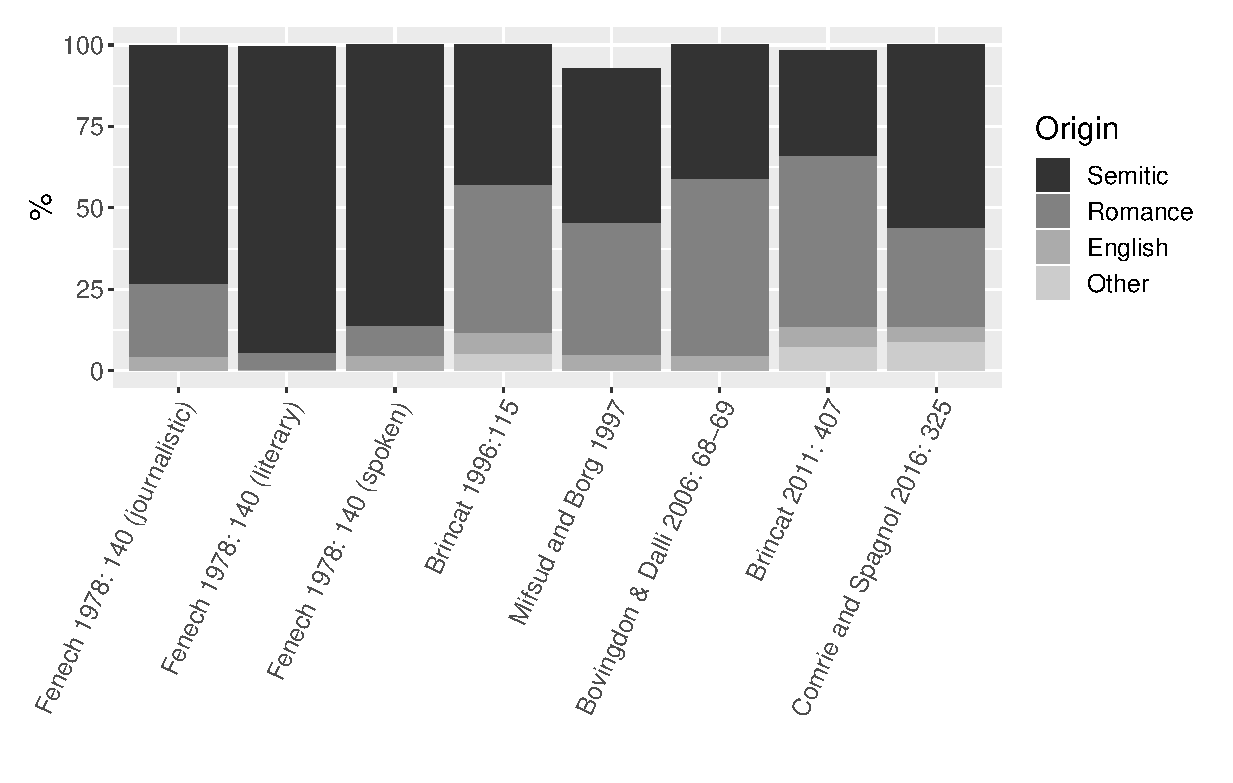
\includegraphics[width=12cm]{figures/lexicon.eps}
\caption{A summary of previous studies of the composition of the Maltese lexicon}
\label{lexicon}
\end{figure}
The primary explanation for the sharp differences between these analyses is methodology: while \cite{fenech1978} analyzes entire texts and thus counts tokens, \cite{brincat1996} (including its updated version in \citealt{brincat2011}) and \cite{bovingdondalli2006} analyze lists of unique words, i.e. types. The later is also true of \cite{mifsudborg1997} and \cite{comriespagnol2016}, except where \cite{brincat1996} uses dictionary data and \cite{bovingdondalli2006} corpus data, \cite{mifsudborg1997} employ a list of lexical items with high frequency of use in daily communication and \cite{comriespagnol2016} base their analysis on a list compiled for the purposes of cross-linguistic comparison. The high ratio of words of Semitic origin in token-based analyses is thus due to the prevalence of function words, which are overwhelmingly Arabic. The type-based analyses then provide a somewhat more accurate picture of the lexicon as a whole, even though they are not without their problems. Chief among these is the issue of what exactly counts as type, especially with regard to productive derivational affixes, e.g. whether all the words with the prefix \textit{anti-} count as distinct types or not. 

In addition to general analyses, both \cite{bovingdondalli2006} and \cite{comriespagnol2016} also provide breakdowns for individual parts of speech. Unfortunately, these analyses are not comparable, as each has a different focus: Bovingdon \& Dali (\citeyear[71]{bovingdondalli2006}) are interested in the composition of each etymological stock by word class (Table \ref{tab:posbovingdon}).
%table
\begin{table}[H]
\caption{Source language component of Maltese by word class (\citealt[71]{bovingdondalli2006}).}
\label{tab:posbovingdon}
\begin{tabular}{lllllll}
\lsptoprule
Origin & Function words & Verbs & Adjectives & Nouns & Adverbs & Pronouns\\
\midrule
Semitic & \multicolumn{1}{r}{3\%} & \multicolumn{1}{r}{70\%} & \multicolumn{1}{r}{2\%} 
& \multicolumn{1}{r}{21\%} & \multicolumn{1}{r}{2\%} & \multicolumn{1}{r}{2\%} \\
Romance & \multicolumn{1}{r}{0\%} & \multicolumn{1}{r}{38\%} & \multicolumn{1}{r}{11\%} 
& \multicolumn{1}{r}{48\%} & \multicolumn{1}{r}{3\%} & \multicolumn{1}{r}{0\%} \\
English & \multicolumn{1}{r}{0\%} & \multicolumn{1}{r}{29\%} & \multicolumn{1}{r}{8\%} & \multicolumn{1}{r}{63\%}
& \multicolumn{1}{r}{0\%} & \multicolumn{1}{r}{0\%} \\
\lspbottomrule
\end{tabular}
\end{table}
In contrast, Comrie \& Spagnol (\citeyear[328]{comriespagnol2016}) focus on the composition of individual word classes by their origin (Table \ref{tab:comriespagnol}).\footnote{The details of Comrie \& Spagnol's (\citeyear{comriespagnol2016}) methodology mean that loans in their dataset come from Romance and English but not from any other languages. The category we label ``Misc.'' in Tables \ref{tab:comriespagnol} and \ref{tab:comriespagnolsemantic} encompasses those meanings in the \textit{Loanwords in the world's languages} 1500-item set which have no corresponding single-word Maltese lexical item, and those where the etymology is at present unknown, or where the item in question is an innovative Maltese-internal coinage.}
%table
\begin{table}[H]
\caption{Word class composition by source language (\citealt[328]{comriespagnol2016})}
\label{tab:comriespagnol}
\begin{tabular}{lllll}
\lsptoprule
Word class & Arabic & Romance & English & Misc.\\
\midrule
Function words & \multicolumn{1}{r}{84.7\%} & \multicolumn{1}{r}{6.2\%} & \multicolumn{1}{r}{0\%} & \multicolumn{1}{r}{9.1\%} \\
Verbs & \multicolumn{1}{r}{75.3\%} & \multicolumn{1}{r}{14.1\%} & \multicolumn{1}{r}{1.3\%} & \multicolumn{1}{r}{9.2\%} \\
Adjectives & \multicolumn{1}{r}{65.2\%} & \multicolumn{1}{r}{28.5\%} & \multicolumn{1}{r}{0.3\%} & \multicolumn{1}{r}{6.0\%} \\
Nouns & \multicolumn{1}{r}{44.7\%} & \multicolumn{1}{r}{39.6\%} & \multicolumn{1}{r}{7.2\%} & \multicolumn{1}{r}{8.6\%} \\
\lspbottomrule
\end{tabular}
\end{table}

\citet{comriespagnol2016} also provide a breakdown of their data by semantic field, permitting a comparison of the domains in which Romance versus English loans are more or less prominent. A number of generalizations can be made here (see Table \ref{tab:comriespagnolsemantic} for a summary), though ultimately they all follow naturally from the fact that contact with English was more recent, and less intensive, than contact with Sicilian and Italian. 

\begin{table}[H]
\caption{Composition of semantic fields by source language (\citealt[327]{comriespagnol2016})}
\label{tab:comriespagnolsemantic}
\begin{tabular}{lllll}
\lsptoprule
Semantic field & Arabic & Romance & English & Misc.\\
\midrule
Modern world & \multicolumn{1}{r}{3.0\%} & \multicolumn{1}{r}{65.3\%} & \multicolumn{1}{r}{22.8\%} & \multicolumn{1}{r}{9.0\%} \\
Animals & \multicolumn{1}{r}{47.8\%} & \multicolumn{1}{r}{29.1\%} & \multicolumn{1}{r}{13.9\%} & \multicolumn{1}{r}{9.1\%} \\
Clothing and grooming & \multicolumn{1}{r}{38.7\%} & \multicolumn{1}{r}{47.2\%} & \multicolumn{1}{r}{10.4\%} & \multicolumn{1}{r}{3.8\%} \\
Warfare and hunting & \multicolumn{1}{r}{28.8\%} & \multicolumn{1}{r}{65.0\%} & \multicolumn{1}{r}{2.5\%} & \multicolumn{1}{r}{3.8\%} \\
Law & \multicolumn{1}{r}{36.0\%} & \multicolumn{1}{r}{50.0\%} & \multicolumn{1}{r}{0.0\%} & \multicolumn{1}{r}{14.0\%} \\
Social and political relations & \multicolumn{1}{r}{48.4\%} & \multicolumn{1}{r}{48.4\%} & \multicolumn{1}{r}{0.0\%} & \multicolumn{1}{r}{3.2\%} \\
\lspbottomrule
\end{tabular}
\end{table}

Unsurprisingly, English is best represented in the category of items relating to the modern world, but even here Romance dominates. Examples include English-derived \textit{televixin} `television' and Italian-derived \textit{kafè} `coffee'. 

The domain of animals divides rather neatly as follows. Common animals (especially land animals) of the Mediterranean area are largely Arabic-derived (e.g. \textit{fenek} `rabbit' < Maghrebi Arabic \textit{fanak} `fennec fox'), while well-known non-indigenous animals are largely Romance-derived (e.g. \textit{ljunfant} `elephant' < Sic. \textit{liufanti}, the additional /n/ perhaps the result of influence from \textit{ljun} `lion'). More exotic animals, if there is a corresponding Maltese item at all, derive from English (e.g. \textit{tapir} `tapir'). Clothing and grooming presents a similar picture, with Arabic-derived \textit{suf} `wool', Sicilian-derived \textit{ngwanta} `glove', and English-derived \textit{fer} `fur', as does warfare and hunting, with Arabic-derived \textit{sejf} `sword', Sicilian-derived \textit{xkubetta} `gun', and English-derived \textit{senter} `shotgun' (< \textit{centre-breech-loading shotgun}).

The total lack of English loans in the domains of law and social and political relations, at least in Comrie and Spagnol's sample, is remarkable, given the extent to which the English language dominated public life in Malta in the twentieth century. A generalization that underlies this finding is that while English influence is strongest in the spheres of commerce, consumerism and, especially in the 21st century, popular culture (e.g. \textit{vawċer} `voucher', \textit{ċċettja} `to chat'),\footnote{Until at least 1991, when the Maltese government opened up television broadcasting rights to more than just the single state broadcaster TVM, Italian television stations, whose broadcasts from Sicily could be received in Malta, were very widely watched, and there was consequently considerable Italian influence on Maltese popular culture \citep{sammut2007}. This influence has waned considerably at the expense of English and American culture since the advent of broadcast pluralism in Malta, and especially with the rise of cable television and online video streaming.} at least as far as Maltese lexicon is concerned, it has not supplanted Italian in the domains of high culture and the affairs of state (e.g. \textit{gvern} `government' < Italian \textit{governo}, \textit{poeżija} `poem' < Italian \textit{poesia}).

\subsubsection{Minor sources}
Considering its location and the nature of population movements in the Mediterranean, it is hardly surprising that the Maltese lexicon also contains borrowings from languages other than Sicilian, Italian and English. %other romance 
The most obvious of these are borrowings from other Romance languages. First among them, as in other European languages, stands Latin, which provided a large chunk of Maltese scientific and technical vocabulary, whether as terminology (e.g. \textit{ego},  \textit{rektum} or  \textit{sukkursu} `underground water'), biological nomenclature (\textit{fagu} `European beech, \textit{Fagus sylvatica}', \textit{mirla} `brown wrasse, \textit{Labrus merula}') or set phrases and expressions (\textit{ex cathedra}, \textit{ibidem}). Curiously for a Catholic country, Latin is the source of very little religious vocabulary in Maltese; in this area, Maltese continues to rely almost exclusively on words of Arabic origin. Those Latin words related to religious matters employed in modern Maltese therefore typically refer to minutiae of Catholic Church rituals and procedures, such as \textit{ekseat} `a bishop's permission for a priest to leave the diocese' (< \textit{exeat}) or \textit{indult} `a Pope's authorization to perform an act otherwise not allowed by canon law'. Of the few Latin terms related to religion still in common use, \textit{nobis} stands out as a rather curious lexical item: in Maltese, it is used as a (post-nominal) modifier indicating intensity or size, as in \textit{tkaxkira nobis} `a sound thrashing' or \textit{tindifa nobis} `a thorough cleaning'. 

%Spanish, Catalan and Occitan
Before the Order of Saint John gained control of Malta, the islands were for more than two centuries a part (whether officially or not) of the Crown of Aragon. As such, one would expect that speakers of Maltese during that era found themselves exposed the languages of the Crown like Catalan, Spanish and Occitan, that and this was then reflected in the Maltese lexicon. In truth, however, there are only a few Maltese words that can clearly be traced to Ibero-Romance. \cite{catalan2017} identify a number of lexical items with Catalan and/or Occitan origins, but note that many of them can also be found in Sicilian, which in most cases can be clearly determined as the origin of the loan. On the other hand, there are Maltese words of obviously Romance origin whose current shape cannot be easily explained by any of the processes by which Sicilian or Italian words were made to conform to Maltese phonology, and where the Catalan or Occitan origin postulated by \cite{catalan2017} may offer a better explanation than that of ``local formation" resorted to by previous works. These may include: \textit{boxxla} `compass' < Catalan \textit{búixola} vs. Italian \textit{bussola}; \textit{frixa} `pancreas' < Catalan \textit{freixura} `entrails' and even the very frequent \textit{żgur} `certain', which, due to its phonology, especially the /g/ (see §\ref{sec:311}), points to an origin in Catalan \textit{segur} or Spanish \textit{seguro}, rather than to its (Tuscan) Italian or Sicilian cognates, which both feature a /k/ in its place. These and other lexical items, onomastics (see \citealt[46]{catalan2017}), and even usage (such as the ubiquitous Maltese swear word \textit{l-ostja}, literally `the host, sacramental bread', which is very atypical for Italian or Sicilian, but has a counterpart in the Spanish \textit{la hostia}) suggest some influence of Ibero-Romance on Maltese which is yet to be thoroughly researched.

% French
The much shorter French occupation of the Maltese islands left very little linguistic trace, and so it is internationalisms in the semantic field of culture (\textit{bonton} `high society', \textit{etikett} `etiquette'), fashion (\textit{manikin} `manequin') and the culinary arts (\textit{fundan} `fondant', \textit{ragu} `ragout') where French borrowings in Maltese can be found. The few notable exceptions include \textit{berġa} (< \textit{auberge}), the term used for the residences of langues (chapters) of the Order of Saint John. The most prominent of these palaces, \textit{Berġa ta' Kastilja}, now houses the office of the Prime Minister of Malta, for which the term \textit{Berġa} is often used metonymically. The other two Maltese words of French origin still in frequent daily use both happen to be connected to transportation: \textit{xufier} (< \textit{chauffeur}) `driver' and \textit{xarabank} (< \textit{char à bancs}) `bus'. The latter is particularly interesting due to its pronunciation /ʃɐrɐˈbɐnk/, which indicates that it was borrowed directly from French and not from English (which would give /ʃɛrɛˈbɛnk/, as well as for its connection to the French-speaking Maghreb, where the same word was in use; this indicates the possibility that it was brought from there by Maltese expatriates.

%Greek
In addition to Romance languages, post-classical Greek, with its ubiquitous presence all across the Mediterranean (including the neighboring Sicily), could not help but leave a trace on Maltese vocabulary, small though it is. Aquilina (\citeyear[23]{aquilina1976}) gives \textit{Lapsi} `Feast of Ascension' (< \textit{ανάληψη}) as the solitary example of a Maltese religious term not inherited from Christian Arabic or borrowed from Romance languages. The other two examples of Greek loanwords involve a completely different sphere. The first is \textit{ħamallu} `lewd, vulgar person' < Greek \textit{χαμάλης} (\citealt[7781]{megaleksikon1958}). This word may ultimately be traceable to Arabic (through Turkish), as is evident from its other meaning in Greek, namely `porter' (< \textit{ḥammāl}). However, the meaning in which it appears in Maltese is unique to the Greek word, indicating that it was borrowed into Maltese from Greek. The other such term is \textit{vroma} `complete failure, fiasco' which is quite straightforwardly traceable to the Greek \textit{βρόμα/βρώμα} `dirt, filth' (\citealt[1506, 1516]{megaleksikon1958}).

%Berber
With regard to the debates on the origin and history of Maltese, borrowings from other Afro-Asiatic languages have long been at the center of attention of Maltese etymological research. Berber is perhaps the most notorious example here, with a number of items cited as having Berber origins by \cite{colin1957} and Aquilina (\citeyear[25--39]{aquilina1976}). Aquilina's list is an expansion of Colin's and thus both feature the same conspicuous items, which for the most part involve zoology, such as \textit{fekruna} `tortoise' (< \textit{fekrun}, \citealt[553]{naitzerrad2002}) and \textit{gendus} `bull' (< \textit{agenduz}, \citealt[827]{naitzerrad2002}). 
%or botany, e.g. \textit{lellux} "chrysanthemum" (< , \citealt[XXX]{naitzerrad2002}). - Don't know how easily we'll find an authoritative etymology for this: I don't think Nait-Zerrad got that far!
Additionally, Aquilina postulates a Berber origin for a number of lexical items where this seems questionable. In some cases the items in question are obviously Arabic loanwords in Berber (as with \textit{bilħaqq} `by the way', quite transparently from Arabic \textit{b-il-\d{h}aqq} `in truth'). In other cases subsequent research has argued against a Berber origin. For example, while Aquilina identifies \textit{żenbil} `a large carrying basket' as having a Berber origin, Borg (\citeyear[261]{Borg2004}) notes that it can also be found in the Arabic dialect of Aleppo and Arbil, and traces its ultimate origin to Akkadian through Aramaic. A large group of similarities between Maltese and Berber identified by Aquilina involve ``Berber nursery language'', containing items like Berber \textit{papa} `bread' / Maltese \textit{pappa}, Berber \textit{ppspps} or \textit{ppssi} `urine' / Maltese \textit{pixxa}, and Berber \textit{kakka/qaqah} / Maltese \textit{kakka} (both having to do with defecation). These forms are actually attested cross-linguistically (\citealt{ferguson1964}) at least as far north as Slovak (\citealt{ondrackova2010}) and cannot thus be considered loans from Berber. Nevertheless, the fact that there is a Berber lexical component in Maltese is well established, and \cite{Souag2018berber} has shown that it may be larger than previously thought (e.g. his case for the Berber etymology of the frequent adjective \textit{ċkejken} `small').

%Aramaic
Finally, in addition to Berber, Maltese also contains a small number of words that can be reasonably traced back to Aramaic. Along with obsolescent lexical items such as \textit{żenbil} given above or \textit{andar} `threshing floor' (\citealt[116--117]{Behnstedt2005}), this small list includes the frequent verb \textit{xandara} `to broadcast, to spread (news)', otherwise unattested in any other variety of Arabic (\citealt[46]{Borg1996}). This verb is presumably derived from the common Aramaic root \textit{√šdr} `to dispatch, send' with cognates in Mandaic (\citealt[450]{manddic1963}), Jewish Babylonian Aramaic (JBA; \citealt[1112-1113]{sokoloff2002}) and Christian Neo-Aramaic (\citealt[1179]{Khan2008}). The insertion of [n] reflects the dissimilation of the geminated [dd] into [nd] (\citealt[175--176]{Lipinski1997}); the same phenomenon involving the original geminated [bb] can also account for \textit{żenbil} (cf. JBA \textit{zabbīlā}; \citealt[397]{sokoloff2002}). These borrowings could on the one hand strengthen the case for a Levantine substrate in (if not origin of) Maltese, as \cite{Borg1996} insists; on the other hand, some of them can also be found in other North African varieties (\citealt{Behnstedt2005}).

\section{Conclusion}
This chapter has reviewed the extensive changes that have taken place in Maltese as a result of contact with Sicilian, Tuscan Italian, English, and other languages. The changes due to contact with Italo-Romance languages are so striking, especially but by no means only with respect to lexicon, that it is almost misleading to speak of these contacts having changed ``Maltese". Rather it might be argued that it was a Maghrebi Arabic dialect like any other that was subjected to these changes, and that Maltese, the distinct language that its speakers now feel it to be, was what emerged only once these changes were complete. The result is a language in which typically Semitic and typically Indo-European elements exist side-by-side at all linguistic levels.

The elements of contemporary standard Maltese that are the result of contact, summarized in this chapter, are now relatively well understood. But the language has naturally also evolved in numerous ways that owe little or nothing to the effects of contact with other languages. With a few notable exceptions (e.g. \citealt{Borg1978,Vanhove1993}), these changes have received far less attention. A desideratum for future historical linguistic work on Maltese is therefore to redress this imbalance.

Concerning contact-induced change specifically, future research could fruitfully include comparative work on the differential effects of contact on standard versus dialectal Maltese. And to the extent that it is possible, the field would benefit greatly from a detailed history of the sociolinguistic effects of language contact in Malta in the early modern period.

\section*{Further reading}
\cite{krier1976} is a short monograph on the influence of Italo-Romance on Maltese phonology, morphology, syntax, and lexicon. \\
\cite{mifsudloanverbs} gives an in-depth description of Maltese loaned verbs. \\
\cite{comriespagnol2016} examine lexical borrowing in Maltese in the context of loanword typology crosslinguistically. \\
\cite{Drewes1994} and \cite{stolz2003} explore the question of whether Maltese is properly labeled a ``mixed language''.
\section*{Abbreviations}

\begin{tabularx}{.45\textwidth}{lQ}
\textsc{1, 2, 3} & 1st, 2nd, 3rd person \\
\textsc{adj} & adjective \\
BCE & before Common Era \\
\textsc BCv3 & Bulbulistan corpus malti v3 \\
CE & Common Era \\
\textsc{comp} & complementizer \\
\textsc{dat} & dative \\
\textsc{def} & definite article \\
\textsc{dem} & demonstrative \\
\textsc{dep} & dependent form \\
DOM & differential object marking \\
\textsc{f} & feminine \\
JBA & Jewish Babylonian Aramaic \\
\textsc{gen} & genitive \\
\textsc{impf} & imperfect (prefix conjugation) \\
\textsc{inf} & infinitive \\
It. & Italian \\
\textsc{prg} & pragmatic marker \\
\end{tabularx}
\begin{tabularx}{.45\textwidth}{lQ}
\textsc{L1, L2} & 1st, 2nd language \\
\textsc{m} & masculine \\
MUDTv1 & Maltese Universal Dependencies Treebank v1 \\
\textsc{N} & noun \\
\textsc{neg} & negative (particle) \\
NP & noun phrase\\
\textsc{obj} & object \\
\textsc{obl} & oblique \\
\textsc{ptcp} & participle \\
\textsc{pass} & passive \\
\textsc{pl} & plural \\
\textsc{prog} & progressive \\
\textsc{prf} & perfect (suffix conjugation) \\
RL & recipient language \\
Sic. & sicialian \\
\textsc{sg} & singular \\
\textsc{sing} & singulative \\
SL & source language \\
\end{tabularx}

\section*{Acknowledgments}
The research presented in this chapter was partly funded by a Leadership Fellows grant from the UK Arts and Humanities Research Council, grant number APVV-15-0030 from The Slovak Research and Development Agency (APVV), and the ERC Starting Grant number 679083 from the European Research Council, whose support is hereby gratefully acknowledged.
%%% comment by S
%%% added my affiliation stuff
%%% also fixed a typo

\section*{Primary sources}
Maltese examples above are primarily cited from the general corpus of Maltese \textit{bulbulistan corpus malti v3} (accessible at www.bulbul.sk/bonito2, login: guest, password: Ghilm3), as well as from the \textit{Maltese Universal Dependencies Treebank v1} (accessible at www.bulbul.sk/annis-gui-3.4.4/), both described as to their composition and annotation in \cite{bulbul2018}. Each citation is accompanied by an abbreviation identifying the source (BCv3 and MUDTv1, respectively), as well as the specific document where it can be found.

\printbibliography[heading=subbibliography,notkeyword=this]

\end{document}
